\documentclass[../../../main.tex]{subfiles}
\begin{document}
At the beginning of the previous section, it was stated that one option to keep the density of points constant in each layer, so in the whole structure, was to remove points under some criteria. 
Once explained and evidenced, the logic implemented to do so, it was seen that the result obtained was not the expected one. 
Hence, the need to find a new method to reduce the density of points was raised, and it was argued that this method cannot be based on removing or moving points to guarantee the fulfilment of the conditions.
Broadly speaking, the procedure explained so far is based on two principles: triangulation of points and generation of vertices from the triangles created. 
It was shown in previous sections that \textit{n} vertices generate approximately \textit{2n} triangles and that for each triangle, a point is generated. 
The aim of the algorithm implemented in the previous section was to reduce the \textit{n} points to \textit{n/2}, but this proved to be useless. 
Therefore, if the number of points cannot be halved, it only remains to be able to halve the number of triangles. 
Thus, as each triangle generates one point, the number of points in the next layer is indirectly reduced.

The task of controlling the number of triangles in a tessellation is very complex. This is because not all geometric figures can be used to tessellate a plane, as not all of them can fill it without leaving empty or overlapping spaces. 
For example, for regular periodic tessellations\footnote{Regular tessellations are those that are made up by regular polygons, all of the same shape. Only equilateral triangles, squares and hexagons can be used.} only three regular tessellations can be created from equilateral triangles, squares, or regular hexagons.
In the case of semi-regular periodic tessellations\footnote{Semi-regular tessellations use more than one regular polygon.}, only eight combinations\footnote{See \href{https://en.wikipedia.org/wiki/Euclidean\_tilings\_by\_convex\_regular\_polygons\#Archimedean,\_uniform\_or\_semiregular\_tilings}{Archimedean, uniform or semiregular tiling}} of figures can be used.
Outside regular tessellation, irregular tessellation offers more options for tiling a plane, as convex and non-convex polygons can be used, although they are still finite. 
Some types of irregular tessellation use a combination of convex and non-convex polygons to tile the plane, such as Polyominoes\footnote{A \href{https://en.wikipedia.org/wiki/Polyomino}{polyomino} is a plane geometric figure formed by joining one or more squares, for example, the figures in the Tetrix game. However, a generic plane figure formed by joining identical polygons is called polyform.}, but usually a combination of a few polygons is used. 
But even using any geometry, not all geometries can tile a plane. And it is impossible to control in advance the number of tiles that will be used to tile a defined domain using only a few types of polygons. 
Therefore, to control the number of tiles needed to tile a plane, as many different polygons must be used as the number of tiles needed, or fewer.
At the time of writing, to the author's knowledge, there is no algorithm capable of tessellating a set of points with a given number of figures. Some algorithms tessellate a domain with many irregular polygons, one example of this is the \href{https://en.wikipedia.org/wiki/Voronoi_diagram}{Voronoi diagram}. 
The Voronoi diagram is capable of controlling the number of polygons generated, since it grows a polygon from each seed. 
But it is not useful in this case because the polygons that generates do not link the points. 
The algorithm proposed is inspired by the Delaunay tessellation and the polyforms. 
The idea behind it is to tile each section with a constant number of polyforms that contain all the points.
To do so, it modifies a Delaunay tessellation until the number of polygons desired is reached.
While it is true that the polyforms generally are made up of identical polygons, the algorithm proposed is not limited to using only one type of polygon.
So, technically, the polygons used could not be considered as polyforms, but the concept is the same.

The algorithm's workflow starts with the Delaunay tessellation of the points in the layer. 
It was chosen due to it is widely used in computational geometry, so it is optimized and has a low computational cost. 
Once the tessellation is obtained, the area of each triangle in the three-dimensional space is calculated. 
This is done to avoid situations where the projection of the triangle would look small due to the orientation of the triangle.
To calculate the area of a generic triangle in three-dimensional space, the Shoelace formula is used:

\begin{equation}
    A=\frac{1}{2} \sum_{i=1}^n\left(x_i y_{i+1}-x_{i+1} y_i\right)=\frac{1}{2} \sum_{i=1}^n\left|\begin{array}{ll}
    x_i & x_{i+1} \\
    y_i & y_{i+1}
    \end{array}\right|
\end{equation}
Where $A$ is the area of the triangle, $n$ is the number of vertices of the triangle, $x_i$ and $y_i$ are the coordinates of the $i$-th vertex of the triangle, and $x_{n+1}$ and $y_{n+1}$ are the coordinates of the following vertex of the triangle. The Shoelace formula requires the vertices to be ordered in a clockwise or counterclockwise direction. 
So, previously to calculate the area of the triangle, the vertices are ordered in a counterclockwise direction by its polar angle, in the plane that contains each triangle, measured from the centroid of the triangle.
The \textcolor{blue}{Figure} \ref{fig:polar_sort} shows an example of the measure of the polar angle of the vertices from the centroid of the triangle. 
To calculate it, the arc tangent of the vector that goes from the centroid to the vertex is used. 
Once the area of each triangle is calculated, they are sorted by their area in increasing order.

\begin{figure}[!htbp]
    \centering
    

\tikzset{every picture/.style={line width=0.75pt}} %set default line width to 0.75pt        

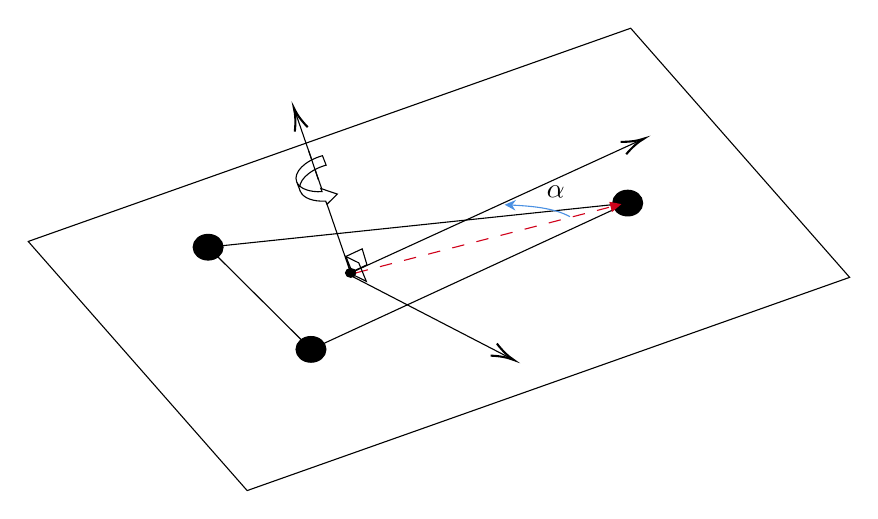
\begin{tikzpicture}[x=0.75pt,y=0.75pt,yscale=-1,xscale=1]
%uncomment if require: \path (0,300); %set diagram left start at 0, and has height of 300

%Shape: Ellipse [id:dp046563370454700936] 
\draw  [fill={rgb, 255:red, 0; green, 0; blue, 0 }  ,fill opacity=1 ] (118.47,120.78) .. controls (118.47,117.36) and (121.7,114.59) .. (125.69,114.59) .. controls (129.67,114.59) and (132.9,117.36) .. (132.9,120.78) .. controls (132.9,124.2) and (129.67,126.97) .. (125.69,126.97) .. controls (121.7,126.97) and (118.47,124.2) .. (118.47,120.78) -- cycle ;
%Shape: Ellipse [id:dp07621414239016377] 
\draw  [fill={rgb, 255:red, 0; green, 0; blue, 0 }  ,fill opacity=1 ] (168.03,170.01) .. controls (168.03,166.59) and (171.26,163.82) .. (175.25,163.82) .. controls (179.23,163.82) and (182.46,166.59) .. (182.46,170.01) .. controls (182.46,173.43) and (179.23,176.2) .. (175.25,176.2) .. controls (171.26,176.2) and (168.03,173.43) .. (168.03,170.01) -- cycle ;
%Shape: Ellipse [id:dp1877409031570847] 
\draw  [fill={rgb, 255:red, 0; green, 0; blue, 0 }  ,fill opacity=1 ] (320.62,99.52) .. controls (320.62,96.1) and (323.86,93.33) .. (327.84,93.33) .. controls (331.83,93.33) and (335.06,96.1) .. (335.06,99.52) .. controls (335.06,102.94) and (331.83,105.71) .. (327.84,105.71) .. controls (323.86,105.71) and (320.62,102.94) .. (320.62,99.52) -- cycle ;
%Straight Lines [id:da09936064873973516] 
\draw    (125.69,120.78) -- (175.25,170.01) ;
%Straight Lines [id:da05718572193121918] 
\draw    (125.69,120.78) -- (327.84,99.52) ;
%Straight Lines [id:da9770419890665386] 
\draw    (175.25,170.01) -- (327.84,99.52) ;
%Shape: Ellipse [id:dp9170551742998044] 
\draw  [color={rgb, 255:red, 0; green, 0; blue, 0 }  ,draw opacity=1 ][fill={rgb, 255:red, 0; green, 0; blue, 0 }  ,fill opacity=1 ] (191.9,133.16) .. controls (191.9,131.98) and (193.01,131.03) .. (194.38,131.03) .. controls (195.74,131.03) and (196.85,131.98) .. (196.85,133.16) .. controls (196.85,134.33) and (195.74,135.28) .. (194.38,135.28) .. controls (193.01,135.28) and (191.9,134.33) .. (191.9,133.16) -- cycle ;
%Straight Lines [id:da7210759333744953] 
\draw    (191.9,133.16) -- (271.22,174.21) ;
\draw [shift={(273,175.13)}, rotate = 207.36] [color={rgb, 255:red, 0; green, 0; blue, 0 }  ][line width=0.75]    (10.93,-3.29) .. controls (6.95,-1.4) and (3.31,-0.3) .. (0,0) .. controls (3.31,0.3) and (6.95,1.4) .. (10.93,3.29)   ;
%Straight Lines [id:da5120234278138571] 
\draw    (194.38,133.16) -- (333.88,69.29) ;
\draw [shift={(335.7,68.46)}, rotate = 155.4] [color={rgb, 255:red, 0; green, 0; blue, 0 }  ][line width=0.75]    (10.93,-3.29) .. controls (6.95,-1.4) and (3.31,-0.3) .. (0,0) .. controls (3.31,0.3) and (6.95,1.4) .. (10.93,3.29)   ;
%Straight Lines [id:da3579413094478969] 
\draw [color={rgb, 255:red, 208; green, 2; blue, 27 }  ,draw opacity=1 ] [dash pattern={on 4.5pt off 4.5pt}]  (196.85,133.16) -- (321.89,100.79) ;
\draw [shift={(324.8,100.04)}, rotate = 165.49] [fill={rgb, 255:red, 208; green, 2; blue, 27 }  ,fill opacity=1 ][line width=0.08]  [draw opacity=0] (5.36,-2.57) -- (0,0) -- (5.36,2.57) -- cycle    ;
%Curve Lines [id:da32741599332926175] 
\draw [color={rgb, 255:red, 74; green, 144; blue, 226 }  ,draw opacity=1 ]   (300.03,106.1) .. controls (292.2,101.7) and (280.67,100.93) .. (271.51,100.46) ;
\draw [shift={(268.56,100.31)}, rotate = 3.01] [fill={rgb, 255:red, 74; green, 144; blue, 226 }  ,fill opacity=1 ][line width=0.08]  [draw opacity=0] (5.36,-2.57) -- (0,0) -- (5.36,2.57) -- (3.56,0) -- cycle    ;
%Straight Lines [id:da8096038051074093] 
\draw    (194.38,133.16) -- (167.65,55.56) ;
\draw [shift={(167,53.67)}, rotate = 71] [color={rgb, 255:red, 0; green, 0; blue, 0 }  ][line width=0.75]    (10.93,-3.29) .. controls (6.95,-1.4) and (3.31,-0.3) .. (0,0) .. controls (3.31,0.3) and (6.95,1.4) .. (10.93,3.29)   ;
%Curve Left Arrow [id:dp031259015950109825] 
\draw  [fill={rgb, 255:red, 255; green, 255; blue, 255 }  ,fill opacity=1 ] (168.34,89.26) .. controls (166.6,84.78) and (172.17,79.15) .. (180.78,76.69) -- (182.55,81.24) .. controls (173.94,83.7) and (168.37,89.33) .. (170.11,93.81) ;\draw  [fill={rgb, 255:red, 255; green, 255; blue, 255 }  ,fill opacity=1 ] (170.11,93.81) .. controls (171.4,97.13) and (176.36,98.89) .. (182.35,98.57) -- (182.94,100.09) -- (187.96,95.19) -- (179.99,92.5) -- (180.58,94.02) .. controls (174.59,94.34) and (169.63,92.58) .. (168.34,89.26)(170.11,93.81) -- (168.34,89.26) ;
%Straight Lines [id:da807731557940086] 
\draw    (174.2,74.5) -- (178.8,88.3) ;
%Shape: Rectangle [id:dp8690019885169661] 
\draw   (39.02,118.01) -- (329.29,15.28) -- (434.77,135.31) -- (144.5,238.04) -- cycle ;
%Shape: Rectangle [id:dp4850654761462362] 
\draw   (201.91,137.23) -- (195.69,134.16) -- (192.05,125.25) -- (198.27,128.33) -- cycle ;
%Shape: Rectangle [id:dp8492811214621624] 
\draw   (202.22,129.26) -- (194.35,132.94) -- (192.05,125.25) -- (199.92,121.57) -- cycle ;

% Text Node
\draw (287.71,90) node [anchor=north west][inner sep=0.75pt]  [rotate=-1.81]  {$\alpha $};


\end{tikzpicture}

    \caption{Illustration of the measure of the polar angle of the vertices from the centroid of the triangle.}
    \label{fig:polar_sort}
\end{figure}

Once all the triangles are sorted by their area, an iterative loop starts merging polygons until the number of polygons desired is reached, which is passed as an argument to the algorithm. 
This loop selects the triangle with the smallest area, which will always be the first element of the sorted list, and looks for its neighbouring triangles. 
To find the neighbouring triangles, the vertices of the triangle are compared with the vertices of the rest of the triangles. 
If two triangles share two vertices, they are considered neighbours. 
Each triangle has three neighbours, except the outer triangles, which have two.
Then, the area of each of the neighbouring triangles is retrieved from the sorted list, and the triangle with the smallest area is merged with the selected triangle.
The area of the new polygon is calculated by adding the area of the two triangles.
And this area is added to the sorted list of areas in the correct position.
Also, the areas of the merged triangles are removed from the list.
So, the new first element will be the current smaller triangle. 
From now on, there won't only be triangles, so the simplices will be called polygons instead of triangles.
This process is repeated until the number of polygons is equal to the initial one, so each layer has the same number of polygons.
The different parts of the algorithm will be explained in detail in the following sections.

\subsection{Merging polygons}

At the beginning of the loop, merging the polygons is a simple task, as all the polygons are triangles. 
But as the number of polygons decreases, the task becomes more complex because the polygons become mainly non-convex.
In fact, there are often situations in which polygons are no longer polygons, since the union between a non-convex polygon and a convex polygon can generate a figure containing points inside it.
One example of this is shown in the \textcolor{blue}{Figure} \ref{fig:merge}.
It should be noted that this is not really a problem since, for the algorithm to work it is only necessary to know the points belonging to each set that represent each of the bases of the future pyramids.
Solving this problem only helps to visually represent the tiling but does not affect the robustness of the algorithm.

\begin{figure}[!htbp]
    \centering
    

% Pattern Info
 
\tikzset{
pattern size/.store in=\mcSize, 
pattern size = 5pt,
pattern thickness/.store in=\mcThickness, 
pattern thickness = 0.3pt,
pattern radius/.store in=\mcRadius, 
pattern radius = 1pt}
\makeatletter
\pgfutil@ifundefined{pgf@pattern@name@_hy82zy3w3}{
\pgfdeclarepatternformonly[\mcThickness,\mcSize]{_hy82zy3w3}
{\pgfqpoint{-\mcThickness}{-\mcThickness}}
{\pgfpoint{\mcSize}{\mcSize}}
{\pgfpoint{\mcSize}{\mcSize}}
{
\pgfsetcolor{\tikz@pattern@color}
\pgfsetlinewidth{\mcThickness}
\pgfpathmoveto{\pgfpointorigin}
\pgfpathlineto{\pgfpoint{0}{\mcSize}}
\pgfusepath{stroke}
}}
\makeatother
\tikzset{every picture/.style={line width=0.75pt}} %set default line width to 0.75pt        

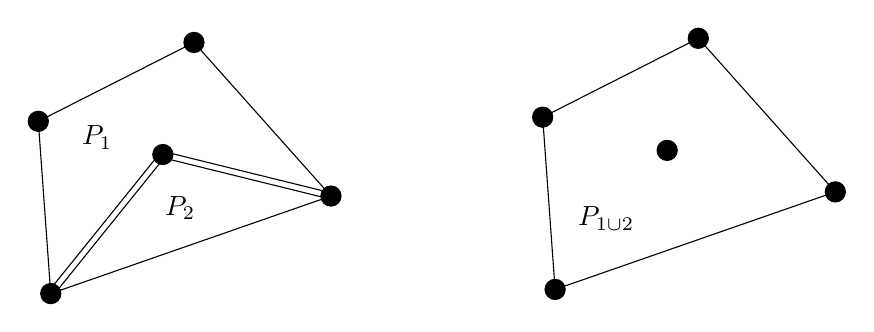
\begin{tikzpicture}[x=0.75pt,y=0.75pt,yscale=-1,xscale=1]
%uncomment if require: \path (0,300); %set diagram left start at 0, and has height of 300

%Shape: Circle [id:dp0903854075610232] 
\draw  [fill={rgb, 255:red, 0; green, 0; blue, 0 }  ,fill opacity=1 ] (106.3,114.85) .. controls (106.3,112.17) and (108.47,110) .. (111.15,110) .. controls (113.83,110) and (116,112.17) .. (116,114.85) .. controls (116,117.53) and (113.83,119.7) .. (111.15,119.7) .. controls (108.47,119.7) and (106.3,117.53) .. (106.3,114.85) -- cycle ;
%Shape: Circle [id:dp3184910134932345] 
\draw  [fill={rgb, 255:red, 0; green, 0; blue, 0 }  ,fill opacity=1 ] (112.3,197.85) .. controls (112.3,195.17) and (114.47,193) .. (117.15,193) .. controls (119.83,193) and (122,195.17) .. (122,197.85) .. controls (122,200.53) and (119.83,202.7) .. (117.15,202.7) .. controls (114.47,202.7) and (112.3,200.53) .. (112.3,197.85) -- cycle ;
%Shape: Circle [id:dp5872048719836919] 
\draw  [fill={rgb, 255:red, 0; green, 0; blue, 0 }  ,fill opacity=1 ] (247.3,150.85) .. controls (247.3,148.17) and (249.47,146) .. (252.15,146) .. controls (254.83,146) and (257,148.17) .. (257,150.85) .. controls (257,153.53) and (254.83,155.7) .. (252.15,155.7) .. controls (249.47,155.7) and (247.3,153.53) .. (247.3,150.85) -- cycle ;
%Shape: Circle [id:dp7591641248768922] 
\draw  [fill={rgb, 255:red, 0; green, 0; blue, 0 }  ,fill opacity=1 ] (181.3,76.85) .. controls (181.3,74.17) and (183.47,72) .. (186.15,72) .. controls (188.83,72) and (191,74.17) .. (191,76.85) .. controls (191,79.53) and (188.83,81.7) .. (186.15,81.7) .. controls (183.47,81.7) and (181.3,79.53) .. (181.3,76.85) -- cycle ;
%Shape: Circle [id:dp7762987079639629] 
\draw  [fill={rgb, 255:red, 0; green, 0; blue, 0 }  ,fill opacity=1 ] (166.3,130.85) .. controls (166.3,128.17) and (168.47,126) .. (171.15,126) .. controls (173.83,126) and (176,128.17) .. (176,130.85) .. controls (176,133.53) and (173.83,135.7) .. (171.15,135.7) .. controls (168.47,135.7) and (166.3,133.53) .. (166.3,130.85) -- cycle ;
%Shape: Circle [id:dp7626801331888498] 
\draw  [fill={rgb, 255:red, 0; green, 0; blue, 0 }  ,fill opacity=1 ] (349.3,112.85) .. controls (349.3,110.17) and (351.47,108) .. (354.15,108) .. controls (356.83,108) and (359,110.17) .. (359,112.85) .. controls (359,115.53) and (356.83,117.7) .. (354.15,117.7) .. controls (351.47,117.7) and (349.3,115.53) .. (349.3,112.85) -- cycle ;
%Shape: Circle [id:dp6435093773617909] 
\draw  [fill={rgb, 255:red, 0; green, 0; blue, 0 }  ,fill opacity=1 ] (355.3,195.85) .. controls (355.3,193.17) and (357.47,191) .. (360.15,191) .. controls (362.83,191) and (365,193.17) .. (365,195.85) .. controls (365,198.53) and (362.83,200.7) .. (360.15,200.7) .. controls (357.47,200.7) and (355.3,198.53) .. (355.3,195.85) -- cycle ;
%Shape: Circle [id:dp23520259436348545] 
\draw  [fill={rgb, 255:red, 0; green, 0; blue, 0 }  ,fill opacity=1 ] (490.3,148.85) .. controls (490.3,146.17) and (492.47,144) .. (495.15,144) .. controls (497.83,144) and (500,146.17) .. (500,148.85) .. controls (500,151.53) and (497.83,153.7) .. (495.15,153.7) .. controls (492.47,153.7) and (490.3,151.53) .. (490.3,148.85) -- cycle ;
%Shape: Circle [id:dp5139999912619062] 
\draw  [fill={rgb, 255:red, 0; green, 0; blue, 0 }  ,fill opacity=1 ] (424.3,74.85) .. controls (424.3,72.17) and (426.47,70) .. (429.15,70) .. controls (431.83,70) and (434,72.17) .. (434,74.85) .. controls (434,77.53) and (431.83,79.7) .. (429.15,79.7) .. controls (426.47,79.7) and (424.3,77.53) .. (424.3,74.85) -- cycle ;
%Shape: Circle [id:dp9128853181814609] 
\draw  [fill={rgb, 255:red, 0; green, 0; blue, 0 }  ,fill opacity=1 ] (409.3,128.85) .. controls (409.3,126.17) and (411.47,124) .. (414.15,124) .. controls (416.83,124) and (419,126.17) .. (419,128.85) .. controls (419,131.53) and (416.83,133.7) .. (414.15,133.7) .. controls (411.47,133.7) and (409.3,131.53) .. (409.3,128.85) -- cycle ;
%Straight Lines [id:da9543502559927777] 
\draw    (111.15,114.85) -- (117.15,197.85) ;
%Straight Lines [id:da6236204803411575] 
\draw    (111.15,114.85) -- (186.15,76.85) ;
%Straight Lines [id:da36073679376855783] 
\draw    (186.15,76.85) -- (252.15,150.85) ;
%Straight Lines [id:da5089280650914181] 
\draw    (171.51,129.39) -- (252.51,149.39)(170.79,132.31) -- (251.79,152.31) ;
%Straight Lines [id:da9757972098601457] 
\draw (172.32,131.79) -- (118.32,198.79)(169.98,129.91) -- (115.98,196.91) ;
%Straight Lines [id:da2697882015737454] 
\draw    (252.15,150.85) -- (117.15,197.85) ;
%Straight Lines [id:da45150527483296576] 
\draw    (354.15,112.85) -- (360.15,195.85) ;
%Straight Lines [id:da030554361443556277] 
\draw    (354.15,112.85) -- (429.15,74.85) ;
%Straight Lines [id:da1930137132355716] 
\draw    (429.15,74.85) -- (495.15,148.85) ;
%Straight Lines [id:da9231067498266883] 
\draw    (360.15,195.85) -- (495.15,148.85) ;

% Text Node
\draw (131,115.85) node [anchor=north west][inner sep=0.75pt]   [align=left] {$\displaystyle P_{1}$};
% Text Node
\draw (171,149.85) node [anchor=north west][inner sep=0.75pt]   [align=left] {$\displaystyle P_{2}$};
% Text Node
\draw (370,154.85) node [anchor=north west][inner sep=0.75pt]   [align=left] {$\displaystyle P_{1\cup 2}$};


\end{tikzpicture}

    \caption{Example of the union between a non-convex polygon and a convex polygon generates a figure that is not a polygon.}
    \label{fig:merge}
\end{figure}

Since there is no implemented algorithm to represent this tessellation, it has to be done by drawing lines between the points in their correct order.
And to do so, the points that make up the polygons must be ordered in the correct order, clockwise or counter-clockwise.
This is not a problem when the polygons are convex, but it is when they are not.
Given a set of points, $V = \{v_1, v_2, ..., v_n\}$, only exists one convex figure that can be formed by them, the convex hull, which is the smallest convex polygon that contains all the points.
But, if the points form a non-convex polygon, many possible polygons can be formed by them.
Therefore, there is no single way to order the points in a non-convex polygon, so they cannot be ordered by their polar angle, because there is no guarantee that the points are ordered in the correct way, or in any other way than by hand.
An example of this is shown in the \textcolor{blue}{Figure} \ref{fig:non_convex}.
Thus, as mentioned above, the points of each triangle in the Delaunay tessellation are ordered clockwise by their polar angle, so that the polygons can be merged while maintaining this order. 
This ensures that the points of the new polygon will be arranged in the desired order.
To facilitate this task, instead of working with the points, their index in the initial list that contains all the points is used.

\begin{figure}[!htbp]
    \centering
    

\tikzset{every picture/.style={line width=0.75pt}} %set default line width to 0.75pt        

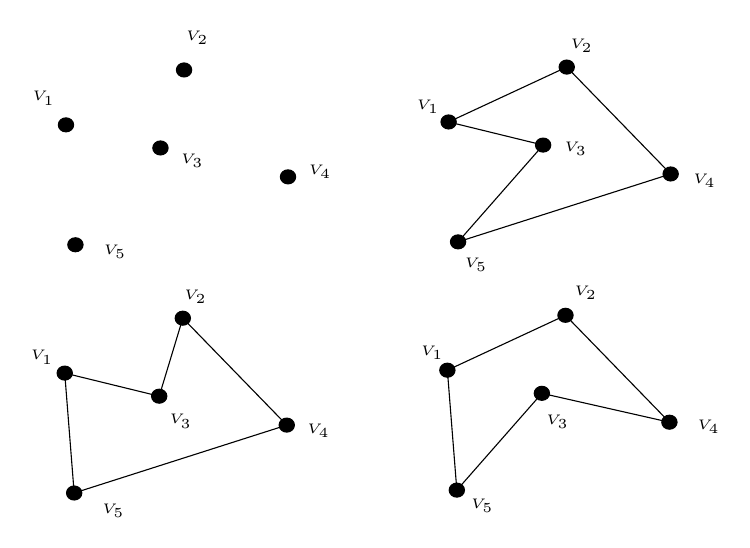
\begin{tikzpicture}[x=0.75pt,y=0.75pt,yscale=-1,xscale=1]
%uncomment if require: \path (0,300); %set diagram left start at 0, and has height of 300

%Shape: Ellipse [id:dp0903854075610232] 
\draw  [fill={rgb, 255:red, 0; green, 0; blue, 0 }  ,fill opacity=1 ] (173.3,63.55) .. controls (173.3,61.69) and (174.95,60.18) .. (176.98,60.18) .. controls (179.01,60.18) and (180.66,61.69) .. (180.66,63.55) .. controls (180.66,65.42) and (179.01,66.93) .. (176.98,66.93) .. controls (174.95,66.93) and (173.3,65.42) .. (173.3,63.55) -- cycle ;
%Shape: Ellipse [id:dp3184910134932345] 
\draw  [fill={rgb, 255:red, 0; green, 0; blue, 0 }  ,fill opacity=1 ] (177.85,121.32) .. controls (177.85,119.46) and (179.5,117.95) .. (181.53,117.95) .. controls (183.56,117.95) and (185.21,119.46) .. (185.21,121.32) .. controls (185.21,123.19) and (183.56,124.7) .. (181.53,124.7) .. controls (179.5,124.7) and (177.85,123.19) .. (177.85,121.32) -- cycle ;
%Shape: Ellipse [id:dp5872048719836919] 
\draw  [fill={rgb, 255:red, 0; green, 0; blue, 0 }  ,fill opacity=1 ] (280.28,88.61) .. controls (280.28,86.75) and (281.92,85.23) .. (283.96,85.23) .. controls (285.99,85.23) and (287.64,86.75) .. (287.64,88.61) .. controls (287.64,90.47) and (285.99,91.99) .. (283.96,91.99) .. controls (281.92,91.99) and (280.28,90.47) .. (280.28,88.61) -- cycle ;
%Shape: Ellipse [id:dp7591641248768922] 
\draw  [fill={rgb, 255:red, 0; green, 0; blue, 0 }  ,fill opacity=1 ] (230.2,37.1) .. controls (230.2,35.24) and (231.85,33.73) .. (233.88,33.73) .. controls (235.91,33.73) and (237.56,35.24) .. (237.56,37.1) .. controls (237.56,38.97) and (235.91,40.48) .. (233.88,40.48) .. controls (231.85,40.48) and (230.2,38.97) .. (230.2,37.1) -- cycle ;
%Shape: Ellipse [id:dp7762987079639629] 
\draw  [fill={rgb, 255:red, 0; green, 0; blue, 0 }  ,fill opacity=1 ] (218.82,74.69) .. controls (218.82,72.82) and (220.47,71.31) .. (222.5,71.31) .. controls (224.53,71.31) and (226.18,72.82) .. (226.18,74.69) .. controls (226.18,76.55) and (224.53,78.06) .. (222.5,78.06) .. controls (220.47,78.06) and (218.82,76.55) .. (218.82,74.69) -- cycle ;
%Shape: Ellipse [id:dp7626801331888498] 
\draw  [fill={rgb, 255:red, 0; green, 0; blue, 0 }  ,fill opacity=1 ] (357.66,62.16) .. controls (357.66,60.29) and (359.31,58.78) .. (361.34,58.78) .. controls (363.38,58.78) and (365.02,60.29) .. (365.02,62.16) .. controls (365.02,64.02) and (363.38,65.54) .. (361.34,65.54) .. controls (359.31,65.54) and (357.66,64.02) .. (357.66,62.16) -- cycle ;
%Shape: Ellipse [id:dp6435093773617909] 
\draw  [fill={rgb, 255:red, 0; green, 0; blue, 0 }  ,fill opacity=1 ] (362.22,119.93) .. controls (362.22,118.07) and (363.86,116.56) .. (365.9,116.56) .. controls (367.93,116.56) and (369.58,118.07) .. (369.58,119.93) .. controls (369.58,121.8) and (367.93,123.31) .. (365.9,123.31) .. controls (363.86,123.31) and (362.22,121.8) .. (362.22,119.93) -- cycle ;
%Shape: Ellipse [id:dp23520259436348545] 
\draw  [fill={rgb, 255:red, 0; green, 0; blue, 0 }  ,fill opacity=1 ] (464.64,87.22) .. controls (464.64,85.35) and (466.29,83.84) .. (468.32,83.84) .. controls (470.35,83.84) and (472,85.35) .. (472,87.22) .. controls (472,89.08) and (470.35,90.59) .. (468.32,90.59) .. controls (466.29,90.59) and (464.64,89.08) .. (464.64,87.22) -- cycle ;
%Shape: Ellipse [id:dp5139999912619062] 
\draw  [fill={rgb, 255:red, 0; green, 0; blue, 0 }  ,fill opacity=1 ] (414.57,35.71) .. controls (414.57,33.84) and (416.21,32.33) .. (418.25,32.33) .. controls (420.28,32.33) and (421.93,33.84) .. (421.93,35.71) .. controls (421.93,37.57) and (420.28,39.09) .. (418.25,39.09) .. controls (416.21,39.09) and (414.57,37.57) .. (414.57,35.71) -- cycle ;
%Shape: Ellipse [id:dp9128853181814609] 
\draw  [fill={rgb, 255:red, 0; green, 0; blue, 0 }  ,fill opacity=1 ] (403.19,73.3) .. controls (403.19,71.43) and (404.83,69.92) .. (406.87,69.92) .. controls (408.9,69.92) and (410.55,71.43) .. (410.55,73.3) .. controls (410.55,75.16) and (408.9,76.67) .. (406.87,76.67) .. controls (404.83,76.67) and (403.19,75.16) .. (403.19,73.3) -- cycle ;
%Straight Lines [id:da45150527483296576] 
\draw    (361.34,62.16) -- (406.87,73.3) ;
%Straight Lines [id:da030554361443556277] 
\draw    (361.34,62.16) -- (418.25,35.71) ;
%Straight Lines [id:da1930137132355716] 
\draw    (418.25,35.71) -- (468.32,87.22) ;
%Straight Lines [id:da9231067498266883] 
\draw    (365.9,119.93) -- (468.32,87.22) ;
%Shape: Ellipse [id:dp4319239618273387] 
\draw  [fill={rgb, 255:red, 0; green, 0; blue, 0 }  ,fill opacity=1 ] (172.7,183.15) .. controls (172.7,181.29) and (174.35,179.78) .. (176.38,179.78) .. controls (178.41,179.78) and (180.06,181.29) .. (180.06,183.15) .. controls (180.06,185.02) and (178.41,186.53) .. (176.38,186.53) .. controls (174.35,186.53) and (172.7,185.02) .. (172.7,183.15) -- cycle ;
%Shape: Ellipse [id:dp7164128195056259] 
\draw  [fill={rgb, 255:red, 0; green, 0; blue, 0 }  ,fill opacity=1 ] (177.25,240.92) .. controls (177.25,239.06) and (178.9,237.55) .. (180.93,237.55) .. controls (182.96,237.55) and (184.61,239.06) .. (184.61,240.92) .. controls (184.61,242.79) and (182.96,244.3) .. (180.93,244.3) .. controls (178.9,244.3) and (177.25,242.79) .. (177.25,240.92) -- cycle ;
%Shape: Ellipse [id:dp9814273885878707] 
\draw  [fill={rgb, 255:red, 0; green, 0; blue, 0 }  ,fill opacity=1 ] (279.68,208.21) .. controls (279.68,206.35) and (281.32,204.83) .. (283.36,204.83) .. controls (285.39,204.83) and (287.04,206.35) .. (287.04,208.21) .. controls (287.04,210.07) and (285.39,211.59) .. (283.36,211.59) .. controls (281.32,211.59) and (279.68,210.07) .. (279.68,208.21) -- cycle ;
%Shape: Ellipse [id:dp9377208715905136] 
\draw  [fill={rgb, 255:red, 0; green, 0; blue, 0 }  ,fill opacity=1 ] (229.6,156.7) .. controls (229.6,154.84) and (231.25,153.33) .. (233.28,153.33) .. controls (235.31,153.33) and (236.96,154.84) .. (236.96,156.7) .. controls (236.96,158.57) and (235.31,160.08) .. (233.28,160.08) .. controls (231.25,160.08) and (229.6,158.57) .. (229.6,156.7) -- cycle ;
%Shape: Ellipse [id:dp30420219582704955] 
\draw  [fill={rgb, 255:red, 0; green, 0; blue, 0 }  ,fill opacity=1 ] (218.22,194.29) .. controls (218.22,192.42) and (219.87,190.91) .. (221.9,190.91) .. controls (223.93,190.91) and (225.58,192.42) .. (225.58,194.29) .. controls (225.58,196.15) and (223.93,197.66) .. (221.9,197.66) .. controls (219.87,197.66) and (218.22,196.15) .. (218.22,194.29) -- cycle ;
%Shape: Ellipse [id:dp6697232002405218] 
\draw  [fill={rgb, 255:red, 0; green, 0; blue, 0 }  ,fill opacity=1 ] (357.06,181.76) .. controls (357.06,179.89) and (358.71,178.38) .. (360.74,178.38) .. controls (362.78,178.38) and (364.42,179.89) .. (364.42,181.76) .. controls (364.42,183.62) and (362.78,185.14) .. (360.74,185.14) .. controls (358.71,185.14) and (357.06,183.62) .. (357.06,181.76) -- cycle ;
%Shape: Ellipse [id:dp3942573514201133] 
\draw  [fill={rgb, 255:red, 0; green, 0; blue, 0 }  ,fill opacity=1 ] (361.62,239.53) .. controls (361.62,237.67) and (363.26,236.16) .. (365.3,236.16) .. controls (367.33,236.16) and (368.98,237.67) .. (368.98,239.53) .. controls (368.98,241.4) and (367.33,242.91) .. (365.3,242.91) .. controls (363.26,242.91) and (361.62,241.4) .. (361.62,239.53) -- cycle ;
%Shape: Ellipse [id:dp991801762708085] 
\draw  [fill={rgb, 255:red, 0; green, 0; blue, 0 }  ,fill opacity=1 ] (464.04,206.82) .. controls (464.04,204.95) and (465.69,203.44) .. (467.72,203.44) .. controls (469.75,203.44) and (471.4,204.95) .. (471.4,206.82) .. controls (471.4,208.68) and (469.75,210.19) .. (467.72,210.19) .. controls (465.69,210.19) and (464.04,208.68) .. (464.04,206.82) -- cycle ;
%Shape: Ellipse [id:dp22587871703179985] 
\draw  [fill={rgb, 255:red, 0; green, 0; blue, 0 }  ,fill opacity=1 ] (413.97,155.31) .. controls (413.97,153.44) and (415.61,151.93) .. (417.65,151.93) .. controls (419.68,151.93) and (421.33,153.44) .. (421.33,155.31) .. controls (421.33,157.17) and (419.68,158.69) .. (417.65,158.69) .. controls (415.61,158.69) and (413.97,157.17) .. (413.97,155.31) -- cycle ;
%Shape: Ellipse [id:dp5394518773608862] 
\draw  [fill={rgb, 255:red, 0; green, 0; blue, 0 }  ,fill opacity=1 ] (402.59,192.9) .. controls (402.59,191.03) and (404.23,189.52) .. (406.27,189.52) .. controls (408.3,189.52) and (409.95,191.03) .. (409.95,192.9) .. controls (409.95,194.76) and (408.3,196.27) .. (406.27,196.27) .. controls (404.23,196.27) and (402.59,194.76) .. (402.59,192.9) -- cycle ;
%Straight Lines [id:da30052767091565935] 
\draw    (176.38,183.15) -- (180.93,240.92) ;
%Straight Lines [id:da045332267906341595] 
\draw    (176.38,183.15) -- (221.9,194.29) ;
%Straight Lines [id:da006754746917110088] 
\draw    (233.28,156.7) -- (283.36,208.21) ;
%Straight Lines [id:da9808534458563097] 
\draw    (283.36,208.21) -- (180.93,240.92) ;
%Straight Lines [id:da7788956384610358] 
\draw    (360.74,181.76) -- (365.3,239.53) ;
%Straight Lines [id:da24525394239037623] 
\draw    (360.74,181.76) -- (417.65,155.31) ;
%Straight Lines [id:da15224280273103452] 
\draw    (417.65,155.31) -- (467.72,206.82) ;
%Straight Lines [id:da7264188286372529] 
\draw    (365.3,239.53) -- (406.27,192.9) ;
%Straight Lines [id:da18718151665886473] 
\draw    (406.87,73.3) -- (365.9,119.93) ;
%Straight Lines [id:da8596127984251889] 
\draw    (233.28,156.7) -- (221.9,194.29) ;
%Straight Lines [id:da67879921706725] 
\draw    (467.72,206.82) -- (406.27,192.9) ;

% Text Node
\draw (159.6,46.2) node [anchor=north west][inner sep=0.75pt]  [font=\tiny] [align=left] {$\displaystyle {\displaystyle V_{1}}$};
% Text Node
\draw (194,120.2) node [anchor=north west][inner sep=0.75pt]  [font=\tiny] [align=left] {$\displaystyle {\displaystyle V_{5}}$};
% Text Node
\draw (231.2,76.2) node [anchor=north west][inner sep=0.75pt]  [font=\tiny] [align=left] {$\displaystyle {\displaystyle V_{3}}$};
% Text Node
\draw (292.8,81.8) node [anchor=north west][inner sep=0.75pt]  [font=\tiny] [align=left] {$\displaystyle {\displaystyle V_{4}}$};
% Text Node
\draw (233.6,17) node [anchor=north west][inner sep=0.75pt]  [font=\tiny] [align=left] {$\displaystyle {\displaystyle V_{2}}$};
% Text Node
\draw (344.8,50.2) node [anchor=north west][inner sep=0.75pt]  [font=\tiny] [align=left] {$\displaystyle {\displaystyle V_{1}}$};
% Text Node
\draw (367.9,126.31) node [anchor=north west][inner sep=0.75pt]  [font=\tiny] [align=left] {$\displaystyle {\displaystyle V_{5}}$};
% Text Node
\draw (416,70.6) node [anchor=north west][inner sep=0.75pt]  [font=\tiny] [align=left] {$\displaystyle {\displaystyle V_{3}}$};
% Text Node
\draw (478,85.8) node [anchor=north west][inner sep=0.75pt]  [font=\tiny] [align=left] {$\displaystyle {\displaystyle V_{4}}$};
% Text Node
\draw (418.8,21) node [anchor=north west][inner sep=0.75pt]  [font=\tiny] [align=left] {$\displaystyle {\displaystyle V_{2}}$};
% Text Node
\draw (346.8,169) node [anchor=north west][inner sep=0.75pt]  [font=\tiny] [align=left] {$\displaystyle {\displaystyle V_{1}}$};
% Text Node
\draw (370.98,242.53) node [anchor=north west][inner sep=0.75pt]  [font=\tiny] [align=left] {$\displaystyle {\displaystyle V_{5}}$};
% Text Node
\draw (407.2,202.2) node [anchor=north west][inner sep=0.75pt]  [font=\tiny] [align=left] {$\displaystyle {\displaystyle V_{3}}$};
% Text Node
\draw (480,204.6) node [anchor=north west][inner sep=0.75pt]  [font=\tiny] [align=left] {$\displaystyle {\displaystyle V_{4}}$};
% Text Node
\draw (420.8,139.8) node [anchor=north west][inner sep=0.75pt]  [font=\tiny] [align=left] {$\displaystyle {\displaystyle V_{2}}$};
% Text Node
\draw (158.8,171) node [anchor=north west][inner sep=0.75pt]  [font=\tiny] [align=left] {$\displaystyle {\displaystyle V_{1}}$};
% Text Node
\draw (193.2,245) node [anchor=north west][inner sep=0.75pt]  [font=\tiny] [align=left] {$\displaystyle {\displaystyle V_{5}}$};
% Text Node
\draw (225.6,201.8) node [anchor=north west][inner sep=0.75pt]  [font=\tiny] [align=left] {$\displaystyle {\displaystyle V_{3}}$};
% Text Node
\draw (292,206.6) node [anchor=north west][inner sep=0.75pt]  [font=\tiny] [align=left] {$\displaystyle {\displaystyle V_{4}}$};
% Text Node
\draw (232.8,141.8) node [anchor=north west][inner sep=0.75pt]  [font=\tiny] [align=left] {$\displaystyle {\displaystyle V_{2}}$};


\end{tikzpicture}

    \caption{Example of the different non-convex polygons that can be obtained from a set of points.}
    \label{fig:non_convex}
\end{figure}

\newpage
The following is the procedure followed to merge the polygons in all possible cases:

\subsubsection*{One common edge}

This is the simplest case. To facilitate the explanation, the polygons will be called $A$ and $B$, where $A$ will always be the polygon with the smallest area and $B$ the neighbour of $A$ to be merged.
Therefore, the common points will be referred to as $A$ and the non-common points as $B$.
The first step is to find which are the common and uncommon indices between the two polygons.
Once the common indices have been identified, the indices of $B$ must be inserted between the common values of $A$. For example, in the \textcolor{blue}{Figure} \ref{fig:merge_1}, a possible case is shown. 
The common indices are $[3,2]$ and the non-common, to be inserted, in $B$ are $[4,1]$.
Then, the position of the first common index, $[3]$, is identified in $A$. 
And after this, all the non-common points present in $B$ are inserted.
The order of the points in each of their sets must be preserved in the final set. 
That is, once the positions of the common values in B have been obtained, the uncommon values must be extracted.
To do so, the index of the first common value on the list is obtained, and the list of indices is shifted by this number of positions.
Obtaining, thus, a list of indices where the first two elements are the common ones and the following ones are the non-common.
Since the indices were ordered clockwise before, the non-common values will also be sorted the same way and, therefore, ready to be inserted into the list of indices of A.
In the example, it would seem logical to eliminate the common points, [2,3], and insert the remaining ones, [1,4], in A. 
But if this is done, the resulting polygon would not be ordered. 
Proceeding as stated, the result in the example would be [4,1]. 
Also, it should be noted that the first common point, $3$, may be in the last position and, therefore, the second common point, $2$, would be in the first position. 
In that case, the intersection between the two sets would appear as $[2,3]$ instead of $[3,2]$, since it is returned according to the order of appearance in the first set. 
Therefore, a pre-insertion step must be added to calculate whether indices are consecutive in the list. 
If they are, the uncommon indices are inserted after the first common index.
If not, they are placed after the second one, which should be the first one. 
That is, if $A$ is $[2,5,3]$ and $B$ is $[1,2,3,4]$, the result must be $[2,5,3,4,1]$ and not $[2,4,1,5,3]$, otherwise the points won't be ordered.
If the points are followed in order, from left to right, one can be able to see it.

\begin{figure}[!htbp]
    \centering
    

\tikzset{every picture/.style={line width=0.75pt}} %set default line width to 0.75pt        

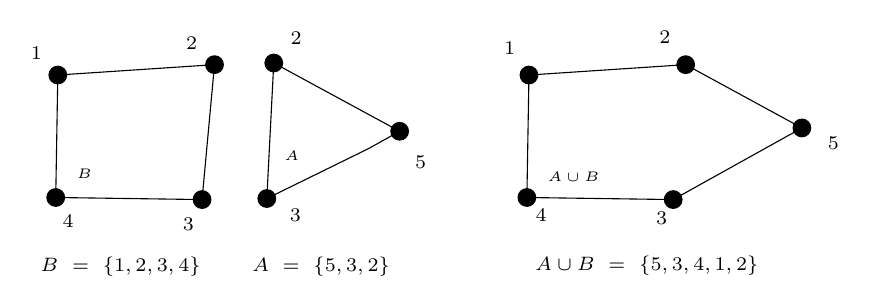
\begin{tikzpicture}[x=0.75pt,y=0.75pt,yscale=-1,xscale=1]
%uncomment if require: \path (0,300); %set diagram left start at 0, and has height of 300

%Shape: Circle [id:dp9539685209278904] 
\draw  [fill={rgb, 255:red, 0; green, 0; blue, 0 }  ,fill opacity=1 ] (100.5,116.25) .. controls (100.5,113.9) and (102.4,112) .. (104.75,112) .. controls (107.1,112) and (109,113.9) .. (109,116.25) .. controls (109,118.6) and (107.1,120.5) .. (104.75,120.5) .. controls (102.4,120.5) and (100.5,118.6) .. (100.5,116.25) -- cycle ;
%Shape: Circle [id:dp17195678469286813] 
\draw  [fill={rgb, 255:red, 0; green, 0; blue, 0 }  ,fill opacity=1 ] (265.2,143.35) .. controls (265.2,141) and (267.1,139.1) .. (269.45,139.1) .. controls (271.8,139.1) and (273.7,141) .. (273.7,143.35) .. controls (273.7,145.7) and (271.8,147.6) .. (269.45,147.6) .. controls (267.1,147.6) and (265.2,145.7) .. (265.2,143.35) -- cycle ;
%Shape: Circle [id:dp19801252920337886] 
\draw  [fill={rgb, 255:red, 0; green, 0; blue, 0 }  ,fill opacity=1 ] (170,176.25) .. controls (170,173.9) and (171.9,172) .. (174.25,172) .. controls (176.6,172) and (178.5,173.9) .. (178.5,176.25) .. controls (178.5,178.6) and (176.6,180.5) .. (174.25,180.5) .. controls (171.9,180.5) and (170,178.6) .. (170,176.25) -- cycle ;
%Shape: Circle [id:dp37568788682491183] 
\draw  [fill={rgb, 255:red, 0; green, 0; blue, 0 }  ,fill opacity=1 ] (176,111.25) .. controls (176,108.9) and (177.9,107) .. (180.25,107) .. controls (182.6,107) and (184.5,108.9) .. (184.5,111.25) .. controls (184.5,113.6) and (182.6,115.5) .. (180.25,115.5) .. controls (177.9,115.5) and (176,113.6) .. (176,111.25) -- cycle ;
%Shape: Circle [id:dp4698315500984862] 
\draw  [fill={rgb, 255:red, 0; green, 0; blue, 0 }  ,fill opacity=1 ] (99.5,175.25) .. controls (99.5,172.9) and (101.4,171) .. (103.75,171) .. controls (106.1,171) and (108,172.9) .. (108,175.25) .. controls (108,177.6) and (106.1,179.5) .. (103.75,179.5) .. controls (101.4,179.5) and (99.5,177.6) .. (99.5,175.25) -- cycle ;
%Shape: Circle [id:dp40533910730754974] 
\draw  [fill={rgb, 255:red, 0; green, 0; blue, 0 }  ,fill opacity=1 ] (327.5,116.25) .. controls (327.5,113.9) and (329.4,112) .. (331.75,112) .. controls (334.1,112) and (336,113.9) .. (336,116.25) .. controls (336,118.6) and (334.1,120.5) .. (331.75,120.5) .. controls (329.4,120.5) and (327.5,118.6) .. (327.5,116.25) -- cycle ;
%Shape: Circle [id:dp12505899664115583] 
\draw  [fill={rgb, 255:red, 0; green, 0; blue, 0 }  ,fill opacity=1 ] (459,141.75) .. controls (459,139.4) and (460.9,137.5) .. (463.25,137.5) .. controls (465.6,137.5) and (467.5,139.4) .. (467.5,141.75) .. controls (467.5,144.1) and (465.6,146) .. (463.25,146) .. controls (460.9,146) and (459,144.1) .. (459,141.75) -- cycle ;
%Shape: Circle [id:dp09472536791892694] 
\draw  [fill={rgb, 255:red, 0; green, 0; blue, 0 }  ,fill opacity=1 ] (397,176.25) .. controls (397,173.9) and (398.9,172) .. (401.25,172) .. controls (403.6,172) and (405.5,173.9) .. (405.5,176.25) .. controls (405.5,178.6) and (403.6,180.5) .. (401.25,180.5) .. controls (398.9,180.5) and (397,178.6) .. (397,176.25) -- cycle ;
%Shape: Circle [id:dp3252294956808539] 
\draw  [fill={rgb, 255:red, 0; green, 0; blue, 0 }  ,fill opacity=1 ] (403,111.25) .. controls (403,108.9) and (404.9,107) .. (407.25,107) .. controls (409.6,107) and (411.5,108.9) .. (411.5,111.25) .. controls (411.5,113.6) and (409.6,115.5) .. (407.25,115.5) .. controls (404.9,115.5) and (403,113.6) .. (403,111.25) -- cycle ;
%Shape: Circle [id:dp2031435773116963] 
\draw  [fill={rgb, 255:red, 0; green, 0; blue, 0 }  ,fill opacity=1 ] (326.5,175.25) .. controls (326.5,172.9) and (328.4,171) .. (330.75,171) .. controls (333.1,171) and (335,172.9) .. (335,175.25) .. controls (335,177.6) and (333.1,179.5) .. (330.75,179.5) .. controls (328.4,179.5) and (326.5,177.6) .. (326.5,175.25) -- cycle ;
%Straight Lines [id:da06021171509697276] 
\draw    (104.75,116.25) -- (103.75,175.25) ;
%Straight Lines [id:da68363488855261] 
\draw    (104.75,116.25) -- (180.25,111.25) ;
%Straight Lines [id:da9736189563059668] 
\draw    (174.25,176.25) -- (103.75,175.25) ;
%Straight Lines [id:da23990827755694877] 
\draw    (174.25,176.25) -- (180.25,111.25) ;
%Straight Lines [id:da7381727541125543] 
\draw    (269.45,143.35) -- (208.8,110.45) ;
%Straight Lines [id:da6555840020070562] 
\draw    (269.45,143.35) -- (254.39,151.73) -- (205.45,175.75) ;
%Shape: Circle [id:dp1876531522593874] 
\draw  [fill={rgb, 255:red, 0; green, 0; blue, 0 }  ,fill opacity=1 ] (204.55,110.45) .. controls (204.55,108.1) and (206.45,106.2) .. (208.8,106.2) .. controls (211.15,106.2) and (213.05,108.1) .. (213.05,110.45) .. controls (213.05,112.8) and (211.15,114.7) .. (208.8,114.7) .. controls (206.45,114.7) and (204.55,112.8) .. (204.55,110.45) -- cycle ;
%Shape: Circle [id:dp6725433808016669] 
\draw  [fill={rgb, 255:red, 0; green, 0; blue, 0 }  ,fill opacity=1 ] (201.2,175.75) .. controls (201.2,173.4) and (203.1,171.5) .. (205.45,171.5) .. controls (207.8,171.5) and (209.7,173.4) .. (209.7,175.75) .. controls (209.7,178.1) and (207.8,180) .. (205.45,180) .. controls (203.1,180) and (201.2,178.1) .. (201.2,175.75) -- cycle ;
%Straight Lines [id:da18786844930320812] 
\draw    (205.45,175.75) -- (208.8,110.45) ;
%Straight Lines [id:da4381692484304286] 
\draw    (331.75,116.25) -- (407.25,111.25) ;
%Straight Lines [id:da3630209393980691] 
\draw    (407.25,111.25) -- (463.25,141.75) ;
%Straight Lines [id:da3559676303350452] 
\draw    (401.25,176.25) -- (463.25,141.75) ;
%Straight Lines [id:da9979085391368497] 
\draw    (330.75,175.25) -- (401.25,176.25) ;
%Straight Lines [id:da7560050387415354] 
\draw    (331.75,116.25) -- (330.75,175.25) ;

% Text Node
\draw (90.5,101.7) node [anchor=north west][inner sep=0.75pt]  [font=\scriptsize] [align=left] {1};
% Text Node
\draw (275.7,154.1) node [anchor=north west][inner sep=0.75pt]  [font=\scriptsize] [align=left] {5};
% Text Node
\draw (105.75,182.5) node [anchor=north west][inner sep=0.75pt]  [font=\scriptsize] [align=left] {4};
% Text Node
\draw (163.7,183.7) node [anchor=north west][inner sep=0.75pt]  [font=\scriptsize] [align=left] {3};
% Text Node
\draw (165.3,96.5) node [anchor=north west][inner sep=0.75pt]  [font=\scriptsize] [align=left] {2};
% Text Node
\draw (215.3,179.7) node [anchor=north west][inner sep=0.75pt]  [font=\scriptsize] [align=left] {3};
% Text Node
\draw (215.7,94.1) node [anchor=north west][inner sep=0.75pt]  [font=\scriptsize] [align=left] {2};
% Text Node
\draw (318.5,98.9) node [anchor=north west][inner sep=0.75pt]  [font=\scriptsize] [align=left] {1};
% Text Node
\draw (333.75,179.7) node [anchor=north west][inner sep=0.75pt]  [font=\scriptsize] [align=left] {4};
% Text Node
\draw (391.7,180.9) node [anchor=north west][inner sep=0.75pt]  [font=\scriptsize] [align=left] {3};
% Text Node
\draw (393.3,93.7) node [anchor=north west][inner sep=0.75pt]  [font=\scriptsize] [align=left] {2};
% Text Node
\draw (474.5,144.9) node [anchor=north west][inner sep=0.75pt]  [font=\scriptsize] [align=left] {5};
% Text Node
\draw (212.8,151.5) node [anchor=north west][inner sep=0.75pt]  [font=\tiny] [align=left] {$\displaystyle A$};
% Text Node
\draw (112.7,160.1) node [anchor=north west][inner sep=0.75pt]  [font=\tiny] [align=left] {$\displaystyle B$};
% Text Node
\draw (339.6,161.8) node [anchor=north west][inner sep=0.75pt]  [font=\tiny] [align=left] {$\displaystyle A\cup B$};
% Text Node
\draw (95.2,202.8) node [anchor=north west][inner sep=0.75pt]  [font=\scriptsize] [align=left] {$\displaystyle B\ =\ \{1,2,3,4\}$};
% Text Node
\draw (197.2,202.8) node [anchor=north west][inner sep=0.75pt]  [font=\scriptsize] [align=left] {$\displaystyle A\ =\ \{5,3,2\}$};
% Text Node
\draw (333.6,202) node [anchor=north west][inner sep=0.75pt]  [font=\scriptsize] [align=left] {$\displaystyle A\cup B\ =\ \{5,3,4,1,2\}$};


\end{tikzpicture}

    \caption{Example of the union between two polygons that share an edge.}
    \label{fig:merge_1}
\end{figure}

\subsubsection*{More than one common edge}

When more than one edge is shared between two polygons, the task becomes more complex. 
The union of the polygons will generate a figure that is not a polygon, as shown in the \textcolor{blue}{Figure} \ref{fig:merge}, regardless of the number of shared edges.
Due to the large number of different possible casuistries, no visually comprehensible way of representing this linkage was found. 
Therefore, it was decided that the best way to deal with these cases is to insert the uncommon values after the first common value, keeping the correct order. 
After the inserted values the last common value is added, and finally, the common values, which are neither the first nor the last, are added at the end of the list. 
This does not allow the figure to be represented as it is, but by relying on the neighbouring polygons, they help to complete the hull of the figure visually. 
However, this is not always the case when the number of shared sides is large. 
Despite this, it should be re-emphasised that this does not affect the robustness of the algorithm as it only compromises the visualization of the tiling.
An example of one of these cases is shown in the \textcolor{blue}{Figure} \ref{fig:merge_2} \textcolor{blue}{A}. 
There, the common indices are $[5,4,3]$ and the uncommon ones are $[1,2]$.
So, the non-commons are inserted after the first common index, $5$, the common indices that are neither the first neither the last, $[4]$ in the example, are added at the end. 
When representing these figures, the first element of the list is replicated at the end of the list to close the figure, as shown in the \textcolor{blue}{Figure} \ref{fig:merge_2} \textcolor{blue}{B}.
The edge between $6$ and $5$ is not represented in the figure, but since this figure will have a neighbouring polygon that will have this edge, it will be represented in the final figure.

\begin{figure}[!htbp]
    \centering
    

\tikzset{every picture/.style={line width=0.75pt}} %set default line width to 0.75pt        

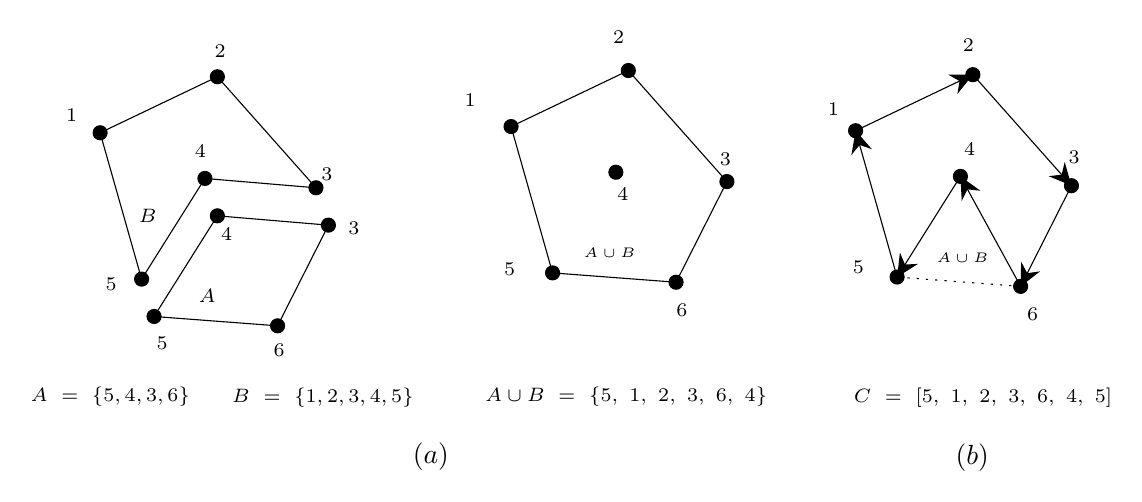
\begin{tikzpicture}[x=0.75pt,y=0.75pt,yscale=-1,xscale=1]
%uncomment if require: \path (0,300); %set diagram left start at 0, and has height of 300

%Shape: Circle [id:dp13697713918046373] 
\draw  [fill={rgb, 255:red, 0; green, 0; blue, 0 }  ,fill opacity=1 ] (84.75,62.38) .. controls (84.75,60.51) and (86.26,59) .. (88.13,59) .. controls (89.99,59) and (91.5,60.51) .. (91.5,62.38) .. controls (91.5,64.24) and (89.99,65.75) .. (88.13,65.75) .. controls (86.26,65.75) and (84.75,64.24) .. (84.75,62.38) -- cycle ;
%Shape: Circle [id:dp8505726277522575] 
\draw  [fill={rgb, 255:red, 0; green, 0; blue, 0 }  ,fill opacity=1 ] (110.75,150.88) .. controls (110.75,149.01) and (112.26,147.5) .. (114.13,147.5) .. controls (115.99,147.5) and (117.5,149.01) .. (117.5,150.88) .. controls (117.5,152.74) and (115.99,154.25) .. (114.13,154.25) .. controls (112.26,154.25) and (110.75,152.74) .. (110.75,150.88) -- cycle ;
%Shape: Circle [id:dp6957030526501801] 
\draw  [fill={rgb, 255:red, 0; green, 0; blue, 0 }  ,fill opacity=1 ] (135.25,84.38) .. controls (135.25,82.51) and (136.76,81) .. (138.63,81) .. controls (140.49,81) and (142,82.51) .. (142,84.38) .. controls (142,86.24) and (140.49,87.75) .. (138.63,87.75) .. controls (136.76,87.75) and (135.25,86.24) .. (135.25,84.38) -- cycle ;
%Shape: Circle [id:dp3439063051120669] 
\draw  [fill={rgb, 255:red, 0; green, 0; blue, 0 }  ,fill opacity=1 ] (188.75,88.88) .. controls (188.75,87.01) and (190.26,85.5) .. (192.13,85.5) .. controls (193.99,85.5) and (195.5,87.01) .. (195.5,88.88) .. controls (195.5,90.74) and (193.99,92.25) .. (192.13,92.25) .. controls (190.26,92.25) and (188.75,90.74) .. (188.75,88.88) -- cycle ;
%Shape: Circle [id:dp9704095790958681] 
\draw  [fill={rgb, 255:red, 0; green, 0; blue, 0 }  ,fill opacity=1 ] (141.25,35.38) .. controls (141.25,33.51) and (142.76,32) .. (144.63,32) .. controls (146.49,32) and (148,33.51) .. (148,35.38) .. controls (148,37.24) and (146.49,38.75) .. (144.63,38.75) .. controls (142.76,38.75) and (141.25,37.24) .. (141.25,35.38) -- cycle ;
%Shape: Circle [id:dp25998291130696727] 
\draw  [fill={rgb, 255:red, 0; green, 0; blue, 0 }  ,fill opacity=1 ] (104.75,132.88) .. controls (104.75,131.01) and (106.26,129.5) .. (108.13,129.5) .. controls (109.99,129.5) and (111.5,131.01) .. (111.5,132.88) .. controls (111.5,134.74) and (109.99,136.25) .. (108.13,136.25) .. controls (106.26,136.25) and (104.75,134.74) .. (104.75,132.88) -- cycle ;
%Shape: Circle [id:dp2350631327028263] 
\draw  [fill={rgb, 255:red, 0; green, 0; blue, 0 }  ,fill opacity=1 ] (141.25,102.38) .. controls (141.25,100.51) and (142.76,99) .. (144.63,99) .. controls (146.49,99) and (148,100.51) .. (148,102.38) .. controls (148,104.24) and (146.49,105.75) .. (144.63,105.75) .. controls (142.76,105.75) and (141.25,104.24) .. (141.25,102.38) -- cycle ;
%Shape: Circle [id:dp7827844033831461] 
\draw  [fill={rgb, 255:red, 0; green, 0; blue, 0 }  ,fill opacity=1 ] (194.75,106.88) .. controls (194.75,105.01) and (196.26,103.5) .. (198.13,103.5) .. controls (199.99,103.5) and (201.5,105.01) .. (201.5,106.88) .. controls (201.5,108.74) and (199.99,110.25) .. (198.13,110.25) .. controls (196.26,110.25) and (194.75,108.74) .. (194.75,106.88) -- cycle ;
%Shape: Circle [id:dp5984519628047641] 
\draw  [fill={rgb, 255:red, 0; green, 0; blue, 0 }  ,fill opacity=1 ] (170.25,155.38) .. controls (170.25,153.51) and (171.76,152) .. (173.63,152) .. controls (175.49,152) and (177,153.51) .. (177,155.38) .. controls (177,157.24) and (175.49,158.75) .. (173.63,158.75) .. controls (171.76,158.75) and (170.25,157.24) .. (170.25,155.38) -- cycle ;
%Straight Lines [id:da06862524702693684] 
\draw    (88.13,62.38) -- (144.63,35.38) ;
%Straight Lines [id:da9660786684329544] 
\draw    (144.63,35.38) -- (192.13,88.88) ;
%Straight Lines [id:da7348457697602903] 
\draw    (138.63,84.38) -- (192.13,88.88) ;
%Straight Lines [id:da4750360942060473] 
\draw    (138.63,84.38) -- (108.13,132.88) ;
%Straight Lines [id:da6122051730873473] 
\draw    (88.13,62.38) -- (108.13,132.88) ;
%Straight Lines [id:da14464697295758544] 
\draw    (144.63,102.38) -- (114.13,150.88) ;
%Straight Lines [id:da30526871036725645] 
\draw    (144.63,102.38) -- (198.13,106.88) ;
%Straight Lines [id:da9282358610345429] 
\draw    (173.63,155.38) -- (114.13,150.88) ;
%Straight Lines [id:da7128692568004056] 
\draw    (173.63,155.38) -- (198.13,106.88) ;
%Shape: Circle [id:dp8591338688223725] 
\draw  [fill={rgb, 255:red, 0; green, 0; blue, 0 }  ,fill opacity=1 ] (282.75,59.38) .. controls (282.75,57.51) and (284.26,56) .. (286.13,56) .. controls (287.99,56) and (289.5,57.51) .. (289.5,59.38) .. controls (289.5,61.24) and (287.99,62.75) .. (286.13,62.75) .. controls (284.26,62.75) and (282.75,61.24) .. (282.75,59.38) -- cycle ;
%Shape: Circle [id:dp44136628753488827] 
\draw  [fill={rgb, 255:red, 0; green, 0; blue, 0 }  ,fill opacity=1 ] (333.25,81.38) .. controls (333.25,79.51) and (334.76,78) .. (336.63,78) .. controls (338.49,78) and (340,79.51) .. (340,81.38) .. controls (340,83.24) and (338.49,84.75) .. (336.63,84.75) .. controls (334.76,84.75) and (333.25,83.24) .. (333.25,81.38) -- cycle ;
%Shape: Circle [id:dp5197915292676696] 
\draw  [fill={rgb, 255:red, 0; green, 0; blue, 0 }  ,fill opacity=1 ] (386.75,85.88) .. controls (386.75,84.01) and (388.26,82.5) .. (390.13,82.5) .. controls (391.99,82.5) and (393.5,84.01) .. (393.5,85.88) .. controls (393.5,87.74) and (391.99,89.25) .. (390.13,89.25) .. controls (388.26,89.25) and (386.75,87.74) .. (386.75,85.88) -- cycle ;
%Shape: Circle [id:dp2805204502688967] 
\draw  [fill={rgb, 255:red, 0; green, 0; blue, 0 }  ,fill opacity=1 ] (339.25,32.38) .. controls (339.25,30.51) and (340.76,29) .. (342.63,29) .. controls (344.49,29) and (346,30.51) .. (346,32.38) .. controls (346,34.24) and (344.49,35.75) .. (342.63,35.75) .. controls (340.76,35.75) and (339.25,34.24) .. (339.25,32.38) -- cycle ;
%Shape: Circle [id:dp8899258705918431] 
\draw  [fill={rgb, 255:red, 0; green, 0; blue, 0 }  ,fill opacity=1 ] (302.75,129.88) .. controls (302.75,128.01) and (304.26,126.5) .. (306.13,126.5) .. controls (307.99,126.5) and (309.5,128.01) .. (309.5,129.88) .. controls (309.5,131.74) and (307.99,133.25) .. (306.13,133.25) .. controls (304.26,133.25) and (302.75,131.74) .. (302.75,129.88) -- cycle ;
%Shape: Circle [id:dp4722303212665844] 
\draw  [fill={rgb, 255:red, 0; green, 0; blue, 0 }  ,fill opacity=1 ] (362.25,134.38) .. controls (362.25,132.51) and (363.76,131) .. (365.63,131) .. controls (367.49,131) and (369,132.51) .. (369,134.38) .. controls (369,136.24) and (367.49,137.75) .. (365.63,137.75) .. controls (363.76,137.75) and (362.25,136.24) .. (362.25,134.38) -- cycle ;
%Straight Lines [id:da8779034684774795] 
\draw    (286.13,59.38) -- (342.63,32.38) ;
%Straight Lines [id:da5866163501693322] 
\draw    (342.63,32.38) -- (390.13,85.88) ;
%Straight Lines [id:da20891965910292054] 
\draw    (286.13,59.38) -- (306.13,129.88) ;
%Straight Lines [id:da4480795127777464] 
\draw    (365.63,134.38) -- (306.13,129.88) ;
%Straight Lines [id:da4030448761724379] 
\draw    (365.63,134.38) -- (390.13,85.88) ;
%Shape: Circle [id:dp12505357057171118] 
\draw  [fill={rgb, 255:red, 0; green, 0; blue, 0 }  ,fill opacity=1 ] (448.75,61.38) .. controls (448.75,59.51) and (450.26,58) .. (452.13,58) .. controls (453.99,58) and (455.5,59.51) .. (455.5,61.38) .. controls (455.5,63.24) and (453.99,64.75) .. (452.13,64.75) .. controls (450.26,64.75) and (448.75,63.24) .. (448.75,61.38) -- cycle ;
%Shape: Circle [id:dp5746788054186597] 
\draw  [fill={rgb, 255:red, 0; green, 0; blue, 0 }  ,fill opacity=1 ] (499.25,83.38) .. controls (499.25,81.51) and (500.76,80) .. (502.63,80) .. controls (504.49,80) and (506,81.51) .. (506,83.38) .. controls (506,85.24) and (504.49,86.75) .. (502.63,86.75) .. controls (500.76,86.75) and (499.25,85.24) .. (499.25,83.38) -- cycle ;
%Shape: Circle [id:dp09128011464267372] 
\draw  [fill={rgb, 255:red, 0; green, 0; blue, 0 }  ,fill opacity=1 ] (552.75,87.88) .. controls (552.75,86.01) and (554.26,84.5) .. (556.13,84.5) .. controls (557.99,84.5) and (559.5,86.01) .. (559.5,87.88) .. controls (559.5,89.74) and (557.99,91.25) .. (556.13,91.25) .. controls (554.26,91.25) and (552.75,89.74) .. (552.75,87.88) -- cycle ;
%Shape: Circle [id:dp4758380405926569] 
\draw  [fill={rgb, 255:red, 0; green, 0; blue, 0 }  ,fill opacity=1 ] (505.25,34.38) .. controls (505.25,32.51) and (506.76,31) .. (508.63,31) .. controls (510.49,31) and (512,32.51) .. (512,34.38) .. controls (512,36.24) and (510.49,37.75) .. (508.63,37.75) .. controls (506.76,37.75) and (505.25,36.24) .. (505.25,34.38) -- cycle ;
%Shape: Circle [id:dp46268099577976185] 
\draw  [fill={rgb, 255:red, 0; green, 0; blue, 0 }  ,fill opacity=1 ] (468.75,131.88) .. controls (468.75,130.01) and (470.26,128.5) .. (472.13,128.5) .. controls (473.99,128.5) and (475.5,130.01) .. (475.5,131.88) .. controls (475.5,133.74) and (473.99,135.25) .. (472.13,135.25) .. controls (470.26,135.25) and (468.75,133.74) .. (468.75,131.88) -- cycle ;
%Shape: Circle [id:dp29163272981610444] 
\draw  [fill={rgb, 255:red, 0; green, 0; blue, 0 }  ,fill opacity=1 ] (528.25,136.38) .. controls (528.25,134.51) and (529.76,133) .. (531.63,133) .. controls (533.49,133) and (535,134.51) .. (535,136.38) .. controls (535,138.24) and (533.49,139.75) .. (531.63,139.75) .. controls (529.76,139.75) and (528.25,138.24) .. (528.25,136.38) -- cycle ;
%Straight Lines [id:da32662852992492064] 
\draw    (452.13,61.38) -- (505.92,35.67) ;
\draw [shift={(508.63,34.38)}, rotate = 154.46] [fill={rgb, 255:red, 0; green, 0; blue, 0 }  ][line width=0.08]  [draw opacity=0] (10.72,-5.15) -- (0,0) -- (10.72,5.15) -- (7.12,0) -- cycle    ;
%Straight Lines [id:da7621252383734732] 
\draw    (508.63,34.38) -- (554.13,85.63) ;
\draw [shift={(556.13,87.88)}, rotate = 228.4] [fill={rgb, 255:red, 0; green, 0; blue, 0 }  ][line width=0.08]  [draw opacity=0] (10.72,-5.15) -- (0,0) -- (10.72,5.15) -- (7.12,0) -- cycle    ;
%Straight Lines [id:da6231835233611202] 
\draw    (502.63,83.38) -- (473.72,129.34) ;
\draw [shift={(472.13,131.88)}, rotate = 302.16] [fill={rgb, 255:red, 0; green, 0; blue, 0 }  ][line width=0.08]  [draw opacity=0] (10.72,-5.15) -- (0,0) -- (10.72,5.15) -- (7.12,0) -- cycle    ;
%Straight Lines [id:da5474926953011492] 
\draw    (452.94,64.26) -- (472.13,131.88) ;
\draw [shift={(452.13,61.38)}, rotate = 74.16] [fill={rgb, 255:red, 0; green, 0; blue, 0 }  ][line width=0.08]  [draw opacity=0] (10.72,-5.15) -- (0,0) -- (10.72,5.15) -- (7.12,0) -- cycle    ;
%Straight Lines [id:da651840469987403] 
\draw  [dash pattern={on 0.84pt off 2.51pt}]  (531.63,136.38) -- (472.13,131.88) ;
%Straight Lines [id:da6912887937841965] 
\draw    (532.98,133.7) -- (556.13,87.88) ;
\draw [shift={(531.63,136.38)}, rotate = 296.8] [fill={rgb, 255:red, 0; green, 0; blue, 0 }  ][line width=0.08]  [draw opacity=0] (10.72,-5.15) -- (0,0) -- (10.72,5.15) -- (7.12,0) -- cycle    ;
%Straight Lines [id:da3792915173272351] 
\draw    (504.07,86.01) -- (531.63,136.38) ;
\draw [shift={(502.63,83.38)}, rotate = 61.31] [fill={rgb, 255:red, 0; green, 0; blue, 0 }  ][line width=0.08]  [draw opacity=0] (10.72,-5.15) -- (0,0) -- (10.72,5.15) -- (7.12,0) -- cycle    ;

% Text Node
\draw (262.5,42.5) node [anchor=north west][inner sep=0.75pt]  [font=\scriptsize] [align=left] {1};
% Text Node
\draw (281.5,124) node [anchor=north west][inner sep=0.75pt]  [font=\scriptsize] [align=left] {5};
% Text Node
\draw (132.5,67) node [anchor=north west][inner sep=0.75pt]  [font=\scriptsize] [align=left] {4};
% Text Node
\draw (385.5,71) node [anchor=north west][inner sep=0.75pt]  [font=\scriptsize] [align=left] {3};
% Text Node
\draw (334,12) node [anchor=north west][inner sep=0.75pt]  [font=\scriptsize] [align=left] {2};
% Text Node
\draw (336.13,87.88) node [anchor=north west][inner sep=0.75pt]  [font=\scriptsize] [align=left] {4};
% Text Node
\draw (206.5,104) node [anchor=north west][inner sep=0.75pt]  [font=\scriptsize] [align=left] {3};
% Text Node
\draw (364.5,143.5) node [anchor=north west][inner sep=0.75pt]  [font=\scriptsize] [align=left] {6};
% Text Node
\draw (114.13,159.38) node [anchor=north west][inner sep=0.75pt]  [font=\scriptsize] [align=left] {5};
% Text Node
\draw (437.5,47) node [anchor=north west][inner sep=0.75pt]  [font=\scriptsize] [align=left] {1};
% Text Node
\draw (449.5,123) node [anchor=north west][inner sep=0.75pt]  [font=\scriptsize] [align=left] {5};
% Text Node
\draw (553.5,70) node [anchor=north west][inner sep=0.75pt]  [font=\scriptsize] [align=left] {3};
% Text Node
\draw (502.5,16) node [anchor=north west][inner sep=0.75pt]  [font=\scriptsize] [align=left] {2};
% Text Node
\draw (503.13,66.25) node [anchor=north west][inner sep=0.75pt]  [font=\scriptsize] [align=left] {4};
% Text Node
\draw (533.5,145.5) node [anchor=north west][inner sep=0.75pt]  [font=\scriptsize] [align=left] {6};
% Text Node
\draw (70.5,49.5) node [anchor=north west][inner sep=0.75pt]  [font=\scriptsize] [align=left] {1};
% Text Node
\draw (89.5,131) node [anchor=north west][inner sep=0.75pt]  [font=\scriptsize] [align=left] {5};
% Text Node
\draw (193.5,78) node [anchor=north west][inner sep=0.75pt]  [font=\scriptsize] [align=left] {3};
% Text Node
\draw (142,19) node [anchor=north west][inner sep=0.75pt]  [font=\scriptsize] [align=left] {2};
% Text Node
\draw (145.13,106.88) node [anchor=north west][inner sep=0.75pt]  [font=\scriptsize] [align=left] {4};
% Text Node
\draw (170.5,163) node [anchor=north west][inner sep=0.75pt]  [font=\scriptsize] [align=left] {6};
% Text Node
\draw (134.5,136.5) node [anchor=north west][inner sep=0.75pt]  [font=\scriptsize] [align=left] {$\displaystyle A$};
% Text Node
\draw (105.5,98) node [anchor=north west][inner sep=0.75pt]  [font=\scriptsize] [align=left] {$\displaystyle B$};
% Text Node
\draw (490,119) node [anchor=north west][inner sep=0.75pt]  [font=\tiny] [align=left] {$\displaystyle A\cup B$};
% Text Node
\draw (320,116.5) node [anchor=north west][inner sep=0.75pt]  [font=\tiny] [align=left] {$\displaystyle A\cup B$};
% Text Node
\draw (53.5,183.5) node [anchor=north west][inner sep=0.75pt]  [font=\scriptsize] [align=left] {$\displaystyle A\ =\ \{5,4,3,6\}$};
% Text Node
\draw (150.5,184) node [anchor=north west][inner sep=0.75pt]  [font=\scriptsize] [align=left] {$\displaystyle B\ =\ \{1,2,3,4,5\}$};
% Text Node
\draw (272.5,183.5) node [anchor=north west][inner sep=0.75pt]  [font=\scriptsize] [align=left] {$\displaystyle A\cup B\ =\ \{5,\ 1,\ 2,\ 3,\ 6,\ 4\}$};
% Text Node
\draw (450,184) node [anchor=north west][inner sep=0.75pt]  [font=\scriptsize] [align=left] {$\displaystyle C\ =\ [ 5,\ 1,\ 2,\ 3,\ 6,\ 4,\ 5]$};
% Text Node
\draw (237.5,210.5) node [anchor=north west][inner sep=0.75pt]   [align=left] {$\displaystyle ( a)$};
% Text Node
\draw (499,211) node [anchor=north west][inner sep=0.75pt]   [align=left] {$\displaystyle ( b)$};


\end{tikzpicture}

    \caption{Example of the union between two polygons that share more than one edge.}
    \label{fig:merge_2}
\end{figure}

\subsubsection*{All points in common}

This case is a particular case of the previous one.
Two polygons might share more than one edge, and all the points of one of the polygons are common to the other. In this case, the result is the bigger polygon. An example of this case is shown in the \textcolor{blue}{Figure} \ref{fig:merge_3}.

\begin{figure}[!htbp]
    \centering
    

\tikzset{every picture/.style={line width=0.75pt}} %set default line width to 0.75pt        

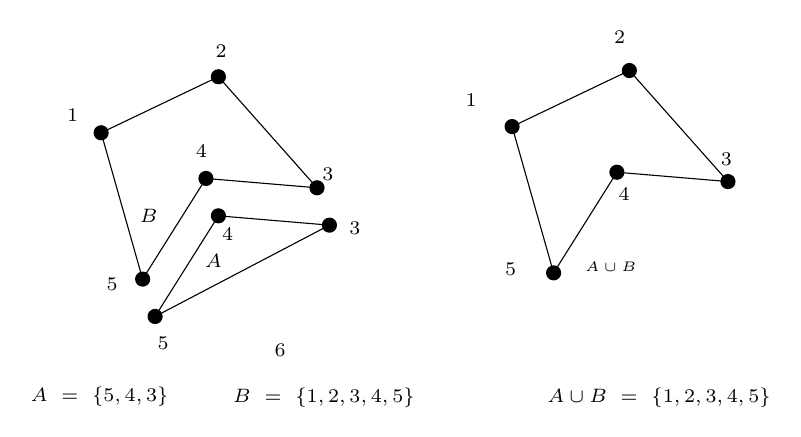
\begin{tikzpicture}[x=0.75pt,y=0.75pt,yscale=-1,xscale=1]
%uncomment if require: \path (0,300); %set diagram left start at 0, and has height of 300

%Shape: Circle [id:dp13697713918046373] 
\draw  [fill={rgb, 255:red, 0; green, 0; blue, 0 }  ,fill opacity=1 ] (84.75,62.38) .. controls (84.75,60.51) and (86.26,59) .. (88.13,59) .. controls (89.99,59) and (91.5,60.51) .. (91.5,62.38) .. controls (91.5,64.24) and (89.99,65.75) .. (88.13,65.75) .. controls (86.26,65.75) and (84.75,64.24) .. (84.75,62.38) -- cycle ;
%Shape: Circle [id:dp8505726277522575] 
\draw  [fill={rgb, 255:red, 0; green, 0; blue, 0 }  ,fill opacity=1 ] (110.75,150.88) .. controls (110.75,149.01) and (112.26,147.5) .. (114.13,147.5) .. controls (115.99,147.5) and (117.5,149.01) .. (117.5,150.88) .. controls (117.5,152.74) and (115.99,154.25) .. (114.13,154.25) .. controls (112.26,154.25) and (110.75,152.74) .. (110.75,150.88) -- cycle ;
%Shape: Circle [id:dp6957030526501801] 
\draw  [fill={rgb, 255:red, 0; green, 0; blue, 0 }  ,fill opacity=1 ] (135.25,84.38) .. controls (135.25,82.51) and (136.76,81) .. (138.63,81) .. controls (140.49,81) and (142,82.51) .. (142,84.38) .. controls (142,86.24) and (140.49,87.75) .. (138.63,87.75) .. controls (136.76,87.75) and (135.25,86.24) .. (135.25,84.38) -- cycle ;
%Shape: Circle [id:dp3439063051120669] 
\draw  [fill={rgb, 255:red, 0; green, 0; blue, 0 }  ,fill opacity=1 ] (188.75,88.88) .. controls (188.75,87.01) and (190.26,85.5) .. (192.13,85.5) .. controls (193.99,85.5) and (195.5,87.01) .. (195.5,88.88) .. controls (195.5,90.74) and (193.99,92.25) .. (192.13,92.25) .. controls (190.26,92.25) and (188.75,90.74) .. (188.75,88.88) -- cycle ;
%Shape: Circle [id:dp9704095790958681] 
\draw  [fill={rgb, 255:red, 0; green, 0; blue, 0 }  ,fill opacity=1 ] (141.25,35.38) .. controls (141.25,33.51) and (142.76,32) .. (144.63,32) .. controls (146.49,32) and (148,33.51) .. (148,35.38) .. controls (148,37.24) and (146.49,38.75) .. (144.63,38.75) .. controls (142.76,38.75) and (141.25,37.24) .. (141.25,35.38) -- cycle ;
%Shape: Circle [id:dp25998291130696727] 
\draw  [fill={rgb, 255:red, 0; green, 0; blue, 0 }  ,fill opacity=1 ] (104.75,132.88) .. controls (104.75,131.01) and (106.26,129.5) .. (108.13,129.5) .. controls (109.99,129.5) and (111.5,131.01) .. (111.5,132.88) .. controls (111.5,134.74) and (109.99,136.25) .. (108.13,136.25) .. controls (106.26,136.25) and (104.75,134.74) .. (104.75,132.88) -- cycle ;
%Shape: Circle [id:dp2350631327028263] 
\draw  [fill={rgb, 255:red, 0; green, 0; blue, 0 }  ,fill opacity=1 ] (141.25,102.38) .. controls (141.25,100.51) and (142.76,99) .. (144.63,99) .. controls (146.49,99) and (148,100.51) .. (148,102.38) .. controls (148,104.24) and (146.49,105.75) .. (144.63,105.75) .. controls (142.76,105.75) and (141.25,104.24) .. (141.25,102.38) -- cycle ;
%Shape: Circle [id:dp7827844033831461] 
\draw  [fill={rgb, 255:red, 0; green, 0; blue, 0 }  ,fill opacity=1 ] (194.75,106.88) .. controls (194.75,105.01) and (196.26,103.5) .. (198.13,103.5) .. controls (199.99,103.5) and (201.5,105.01) .. (201.5,106.88) .. controls (201.5,108.74) and (199.99,110.25) .. (198.13,110.25) .. controls (196.26,110.25) and (194.75,108.74) .. (194.75,106.88) -- cycle ;
%Straight Lines [id:da06862524702693684] 
\draw    (88.13,62.38) -- (144.63,35.38) ;
%Straight Lines [id:da9660786684329544] 
\draw    (144.63,35.38) -- (192.13,88.88) ;
%Straight Lines [id:da7348457697602903] 
\draw    (138.63,84.38) -- (192.13,88.88) ;
%Straight Lines [id:da4750360942060473] 
\draw    (138.63,84.38) -- (108.13,132.88) ;
%Straight Lines [id:da6122051730873473] 
\draw    (88.13,62.38) -- (108.13,132.88) ;
%Straight Lines [id:da14464697295758544] 
\draw    (144.63,102.38) -- (114.13,150.88) ;
%Straight Lines [id:da30526871036725645] 
\draw    (144.63,102.38) -- (198.13,106.88) ;
%Straight Lines [id:da7128692568004056] 
\draw    (114.13,150.88) -- (198.13,106.88) ;
%Shape: Circle [id:dp8591338688223725] 
\draw  [fill={rgb, 255:red, 0; green, 0; blue, 0 }  ,fill opacity=1 ] (282.75,59.38) .. controls (282.75,57.51) and (284.26,56) .. (286.13,56) .. controls (287.99,56) and (289.5,57.51) .. (289.5,59.38) .. controls (289.5,61.24) and (287.99,62.75) .. (286.13,62.75) .. controls (284.26,62.75) and (282.75,61.24) .. (282.75,59.38) -- cycle ;
%Shape: Circle [id:dp44136628753488827] 
\draw  [fill={rgb, 255:red, 0; green, 0; blue, 0 }  ,fill opacity=1 ] (333.25,81.38) .. controls (333.25,79.51) and (334.76,78) .. (336.63,78) .. controls (338.49,78) and (340,79.51) .. (340,81.38) .. controls (340,83.24) and (338.49,84.75) .. (336.63,84.75) .. controls (334.76,84.75) and (333.25,83.24) .. (333.25,81.38) -- cycle ;
%Shape: Circle [id:dp5197915292676696] 
\draw  [fill={rgb, 255:red, 0; green, 0; blue, 0 }  ,fill opacity=1 ] (386.75,85.88) .. controls (386.75,84.01) and (388.26,82.5) .. (390.13,82.5) .. controls (391.99,82.5) and (393.5,84.01) .. (393.5,85.88) .. controls (393.5,87.74) and (391.99,89.25) .. (390.13,89.25) .. controls (388.26,89.25) and (386.75,87.74) .. (386.75,85.88) -- cycle ;
%Shape: Circle [id:dp2805204502688967] 
\draw  [fill={rgb, 255:red, 0; green, 0; blue, 0 }  ,fill opacity=1 ] (339.25,32.38) .. controls (339.25,30.51) and (340.76,29) .. (342.63,29) .. controls (344.49,29) and (346,30.51) .. (346,32.38) .. controls (346,34.24) and (344.49,35.75) .. (342.63,35.75) .. controls (340.76,35.75) and (339.25,34.24) .. (339.25,32.38) -- cycle ;
%Shape: Circle [id:dp8899258705918431] 
\draw  [fill={rgb, 255:red, 0; green, 0; blue, 0 }  ,fill opacity=1 ] (302.75,129.88) .. controls (302.75,128.01) and (304.26,126.5) .. (306.13,126.5) .. controls (307.99,126.5) and (309.5,128.01) .. (309.5,129.88) .. controls (309.5,131.74) and (307.99,133.25) .. (306.13,133.25) .. controls (304.26,133.25) and (302.75,131.74) .. (302.75,129.88) -- cycle ;
%Straight Lines [id:da8779034684774795] 
\draw    (286.13,59.38) -- (342.63,32.38) ;
%Straight Lines [id:da5866163501693322] 
\draw    (342.63,32.38) -- (390.13,85.88) ;
%Straight Lines [id:da20891965910292054] 
\draw    (286.13,59.38) -- (306.13,129.88) ;
%Straight Lines [id:da4030448761724379] 
\draw    (336.63,81.38) -- (390.13,85.88) ;
%Straight Lines [id:da5272117927072546] 
\draw    (336.63,81.38) -- (306.13,129.88) ;

% Text Node
\draw (262.5,42.5) node [anchor=north west][inner sep=0.75pt]  [font=\scriptsize] [align=left] {1};
% Text Node
\draw (281.5,124) node [anchor=north west][inner sep=0.75pt]  [font=\scriptsize] [align=left] {5};
% Text Node
\draw (132.5,67) node [anchor=north west][inner sep=0.75pt]  [font=\scriptsize] [align=left] {4};
% Text Node
\draw (385.5,71) node [anchor=north west][inner sep=0.75pt]  [font=\scriptsize] [align=left] {3};
% Text Node
\draw (334,12) node [anchor=north west][inner sep=0.75pt]  [font=\scriptsize] [align=left] {2};
% Text Node
\draw (336.13,87.88) node [anchor=north west][inner sep=0.75pt]  [font=\scriptsize] [align=left] {4};
% Text Node
\draw (206.5,104) node [anchor=north west][inner sep=0.75pt]  [font=\scriptsize] [align=left] {3};
% Text Node
\draw (114.13,159.38) node [anchor=north west][inner sep=0.75pt]  [font=\scriptsize] [align=left] {5};
% Text Node
\draw (70.5,49.5) node [anchor=north west][inner sep=0.75pt]  [font=\scriptsize] [align=left] {1};
% Text Node
\draw (89.5,131) node [anchor=north west][inner sep=0.75pt]  [font=\scriptsize] [align=left] {5};
% Text Node
\draw (193.5,78) node [anchor=north west][inner sep=0.75pt]  [font=\scriptsize] [align=left] {3};
% Text Node
\draw (142,19) node [anchor=north west][inner sep=0.75pt]  [font=\scriptsize] [align=left] {2};
% Text Node
\draw (145.13,106.88) node [anchor=north west][inner sep=0.75pt]  [font=\scriptsize] [align=left] {4};
% Text Node
\draw (170.5,163) node [anchor=north west][inner sep=0.75pt]  [font=\scriptsize] [align=left] {6};
% Text Node
\draw (137,119.5) node [anchor=north west][inner sep=0.75pt]  [font=\scriptsize] [align=left] {$\displaystyle A$};
% Text Node
\draw (105.5,98) node [anchor=north west][inner sep=0.75pt]  [font=\scriptsize] [align=left] {$\displaystyle B$};
% Text Node
\draw (320,123.5) node [anchor=north west][inner sep=0.75pt]  [font=\tiny] [align=left] {$\displaystyle A\cup B$};
% Text Node
\draw (53,183.5) node [anchor=north west][inner sep=0.75pt]  [font=\scriptsize] [align=left] {$\displaystyle A\ =\ \{5,4,3\}$};
% Text Node
\draw (150.5,184) node [anchor=north west][inner sep=0.75pt]  [font=\scriptsize] [align=left] {$\displaystyle B\ =\ \{1,2,3,4,5\}$};
% Text Node
\draw (302,184) node [anchor=north west][inner sep=0.75pt]  [font=\scriptsize] [align=left] {$\displaystyle A\cup B\ =\ \{1,2,3,4,5\}$};


\end{tikzpicture}

    \caption{Example of the union between two polygons that share all the points.}
    \label{fig:merge_3}
\end{figure}

Once the different cases of merging polygons have been explained, an example of the final tessellation is shown in \textcolor{blue}{Figure} \ref{fig:tessellation_final}.
As it is mentioned above, the final tessellation has as many polygons as the initial points, so the number of polygons is constant in each layer.

\begin{figure}[!htbp]
    \centering
    \includegraphics[width=0.6\textwidth]{imgs/imagenes_numericas.png}
    \caption{Example of the result of the merging polygon process. It can be seen that the number of polygons is constant among the iterations. }
    \label{fig:tessellation_final}
\end{figure}


\subsection{Tetrahedra generation}\label{sec:tetrahedra_gen}

Once the polygons are merged, the next step is to generate the vertices for each polygon.
Since the polygons are not only triangles but a mixture of convex and nonconvex polygons, the vertices cannot be generated by \textcolor{blue}{Equation} \ref{opt:opt_problem}.
The minimisation problem tries to find the point that satisfies the angular conditions with the minimum set of angles and is restricted to a domain that depends on the shape of the base of the polygon.
In the case of a triangle, the domain has a cuboidal shape that stands out the base of the triangle, so the point can be placed anywhere in that cube, and it could be that the projection of the point lies outside the base of the triangle, as it is shown in the \textcolor{blue}{Figure} \ref{fig:optimization}.
This could lead to a situation where the edges of two neighbouring tetrahedra intersect, which is not allowed.
If only convex polygons are considered, this situation is really unlikely to happen because the point that minimises the angles of each edge normally has its projection inside the polygon and close to the centroid of the polygon.
But in the case of non-convex polygons, this situation is really common since the centroid of the polygon is commonly outside the polygon.
To avoid this situation, it is necessary for the vertices to be generated inside the polygon.
In the \textcolor{blue}{Figure} \ref{fig:non_convex_tetra} is shown a possible situation is shown where the tetrahedra are generated from the merged polygon shown in the \textcolor{blue}{Figure} \ref{fig:merge_3}.
To facilitate the comprehension of the figure, an example is shown where the tetrahedra generated are too close to each other, but they do not intersect.
Despite this, this situation is also not allowed since the proximity condition would not be satisfied.
In the figure, the approximated centroid of the polygons is represented as blurred points in the base; the position might not be real, but it helps to visualise the mentioned issue.

\begin{figure}[!htbp]
    \centering
    

\tikzset{every picture/.style={line width=0.75pt}} %set default line width to 0.75pt        

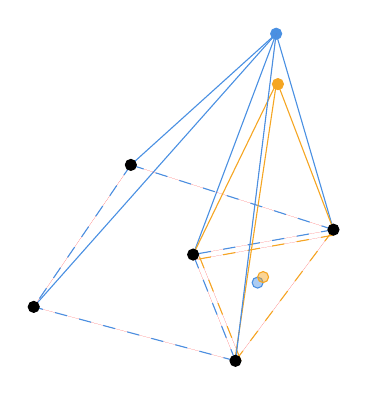
\begin{tikzpicture}[x=0.75pt,y=0.75pt,yscale=-1,xscale=1]
%uncomment if require: \path (0,300); %set diagram left start at 0, and has height of 300

%Shape: Circle [id:dp1755336330892464] 
\draw  [color={rgb, 255:red, 74; green, 144; blue, 226 }  ,draw opacity=1 ][fill={rgb, 255:red, 74; green, 144; blue, 226 }  ,fill opacity=1 ] (252.5,51.15) .. controls (252.5,49.69) and (253.69,48.5) .. (255.15,48.5) .. controls (256.61,48.5) and (257.8,49.69) .. (257.8,51.15) .. controls (257.8,52.61) and (256.61,53.8) .. (255.15,53.8) .. controls (253.69,53.8) and (252.5,52.61) .. (252.5,51.15) -- cycle ;
%Straight Lines [id:da3812362297505554] 
\draw [color={rgb, 255:red, 74; green, 144; blue, 226 }  ,draw opacity=1 ]   (138.35,182.75) -- (255.15,51.15) ;
%Straight Lines [id:da2677948369160592] 
\draw [color={rgb, 255:red, 74; green, 144; blue, 226 }  ,draw opacity=1 ]   (215.15,157.55) -- (255.15,51.15) ;
%Straight Lines [id:da7760470016984858] 
\draw [color={rgb, 255:red, 74; green, 144; blue, 226 }  ,draw opacity=1 ]   (255.15,51.15) -- (185.15,114.35) ;
%Straight Lines [id:da2865796688678216] 
\draw [color={rgb, 255:red, 74; green, 144; blue, 226 }  ,draw opacity=1 ][fill={rgb, 255:red, 254; green, 0; blue, 0 }  ,fill opacity=1 ] [dash pattern={on 4.5pt off 4.5pt}]  (235.55,208.75) -- (138.35,182.75) ;
%Straight Lines [id:da21824910630510064] 
\draw [color={rgb, 255:red, 74; green, 144; blue, 226 }  ,draw opacity=1 ][fill={rgb, 255:red, 254; green, 0; blue, 0 }  ,fill opacity=1 ] [dash pattern={on 4.5pt off 4.5pt}]  (282.75,145.55) -- (185.15,114.35) ;
%Straight Lines [id:da07940346144602317] 
\draw [color={rgb, 255:red, 74; green, 144; blue, 226 }  ,draw opacity=1 ][fill={rgb, 255:red, 254; green, 0; blue, 0 }  ,fill opacity=1 ] [dash pattern={on 4.5pt off 4.5pt}]  (282.75,145.55) -- (215.15,157.55) ;
%Straight Lines [id:da3958333860628518] 
\draw [color={rgb, 255:red, 74; green, 144; blue, 226 }  ,draw opacity=1 ][fill={rgb, 255:red, 254; green, 0; blue, 0 }  ,fill opacity=1 ] [dash pattern={on 4.5pt off 4.5pt}]  (235.55,208.75) -- (215.15,157.55) ;
%Straight Lines [id:da6594564181826876] 
\draw [color={rgb, 255:red, 245; green, 166; blue, 35 }  ,draw opacity=1 ][fill={rgb, 255:red, 254; green, 0; blue, 0 }  ,fill opacity=1 ] [dash pattern={on 4.5pt off 4.5pt}]  (238.2,208.75) -- (217.8,157.55) ;
%Straight Lines [id:da9630174815364824] 
\draw [color={rgb, 255:red, 245; green, 166; blue, 35 }  ,draw opacity=1 ][fill={rgb, 255:red, 254; green, 0; blue, 0 }  ,fill opacity=1 ] [dash pattern={on 4.5pt off 4.5pt}]  (282.75,148.2) -- (215.15,160.2) ;
%Straight Lines [id:da07077764203663617] 
\draw [color={rgb, 255:red, 74; green, 144; blue, 226 }  ,draw opacity=1 ][fill={rgb, 255:red, 254; green, 0; blue, 0 }  ,fill opacity=1 ] [dash pattern={on 4.5pt off 4.5pt}]  (185.15,114.35) -- (138.35,182.75) ;
%Shape: Circle [id:dp21964030873072127] 
\draw  [fill={rgb, 255:red, 0; green, 0; blue, 0 }  ,fill opacity=1 ] (135.7,182.75) .. controls (135.7,181.29) and (136.89,180.1) .. (138.35,180.1) .. controls (139.81,180.1) and (141,181.29) .. (141,182.75) .. controls (141,184.21) and (139.81,185.4) .. (138.35,185.4) .. controls (136.89,185.4) and (135.7,184.21) .. (135.7,182.75) -- cycle ;
%Straight Lines [id:da2086482492059082] 
\draw [color={rgb, 255:red, 74; green, 144; blue, 226 }  ,draw opacity=1 ]   (282.75,145.55) -- (255.15,51.15) ;
%Shape: Circle [id:dp8048871805807353] 
\draw  [fill={rgb, 255:red, 0; green, 0; blue, 0 }  ,fill opacity=1 ] (182.5,114.35) .. controls (182.5,112.89) and (183.69,111.7) .. (185.15,111.7) .. controls (186.61,111.7) and (187.8,112.89) .. (187.8,114.35) .. controls (187.8,115.81) and (186.61,117) .. (185.15,117) .. controls (183.69,117) and (182.5,115.81) .. (182.5,114.35) -- cycle ;
%Straight Lines [id:da28662089505527455] 
\draw [color={rgb, 255:red, 245; green, 166; blue, 35 }  ,draw opacity=1 ][fill={rgb, 255:red, 254; green, 0; blue, 0 }  ,fill opacity=1 ] [dash pattern={on 4.5pt off 4.5pt}]  (235.55,208.75) -- (282.75,145.55) ;
%Shape: Circle [id:dp012864922241068055] 
\draw  [color={rgb, 255:red, 74; green, 144; blue, 226 }  ,draw opacity=1 ][fill={rgb, 255:red, 74; green, 144; blue, 226 }  ,fill opacity=0.46 ] (243.57,171.05) .. controls (243.57,169.59) and (244.75,168.4) .. (246.22,168.4) .. controls (247.68,168.4) and (248.87,169.59) .. (248.87,171.05) .. controls (248.87,172.51) and (247.68,173.7) .. (246.22,173.7) .. controls (244.75,173.7) and (243.57,172.51) .. (243.57,171.05) -- cycle ;
%Shape: Circle [id:dp4580376938600891] 
\draw  [color={rgb, 255:red, 245; green, 166; blue, 35 }  ,draw opacity=1 ][fill={rgb, 255:red, 245; green, 166; blue, 35 }  ,fill opacity=0.48 ] (246.22,168.4) .. controls (246.22,166.94) and (247.4,165.75) .. (248.87,165.75) .. controls (250.33,165.75) and (251.52,166.94) .. (251.52,168.4) .. controls (251.52,169.86) and (250.33,171.05) .. (248.87,171.05) .. controls (247.4,171.05) and (246.22,169.86) .. (246.22,168.4) -- cycle ;
%Shape: Circle [id:dp5893221830726845] 
\draw  [color={rgb, 255:red, 245; green, 166; blue, 35 }  ,draw opacity=1 ][fill={rgb, 255:red, 245; green, 166; blue, 35 }  ,fill opacity=1 ] (253.35,75.42) .. controls (253.35,73.95) and (254.54,72.77) .. (256,72.77) .. controls (257.46,72.77) and (258.65,73.95) .. (258.65,75.42) .. controls (258.65,76.88) and (257.46,78.07) .. (256,78.07) .. controls (254.54,78.07) and (253.35,76.88) .. (253.35,75.42) -- cycle ;
%Straight Lines [id:da7395554317099335] 
\draw [color={rgb, 255:red, 245; green, 166; blue, 35 }  ,draw opacity=1 ]   (215.15,157.55) -- (255,75.58) ;
%Straight Lines [id:da8778033032030901] 
\draw [color={rgb, 255:red, 245; green, 166; blue, 35 }  ,draw opacity=1 ]   (256,75.42) -- (282.75,145.55) ;
%Straight Lines [id:da5166429942869489] 
\draw [color={rgb, 255:red, 245; green, 166; blue, 35 }  ,draw opacity=1 ]   (255.3,74.8) -- (235.05,209.75) ;
%Straight Lines [id:da19726346352627722] 
\draw [color={rgb, 255:red, 74; green, 144; blue, 226 }  ,draw opacity=1 ][fill={rgb, 255:red, 254; green, 0; blue, 0 }  ,fill opacity=1 ]   (235.55,208.75) -- (255.15,51.15) ;
%Shape: Circle [id:dp708841234238893] 
\draw  [fill={rgb, 255:red, 0; green, 0; blue, 0 }  ,fill opacity=1 ] (280.1,145.55) .. controls (280.1,144.09) and (281.29,142.9) .. (282.75,142.9) .. controls (284.21,142.9) and (285.4,144.09) .. (285.4,145.55) .. controls (285.4,147.01) and (284.21,148.2) .. (282.75,148.2) .. controls (281.29,148.2) and (280.1,147.01) .. (280.1,145.55) -- cycle ;
%Shape: Circle [id:dp2885011277156284] 
\draw  [fill={rgb, 255:red, 0; green, 0; blue, 0 }  ,fill opacity=1 ] (212.5,157.55) .. controls (212.5,156.09) and (213.69,154.9) .. (215.15,154.9) .. controls (216.61,154.9) and (217.8,156.09) .. (217.8,157.55) .. controls (217.8,159.01) and (216.61,160.2) .. (215.15,160.2) .. controls (213.69,160.2) and (212.5,159.01) .. (212.5,157.55) -- cycle ;
%Shape: Circle [id:dp8447899615771284] 
\draw  [fill={rgb, 255:red, 0; green, 0; blue, 0 }  ,fill opacity=1 ] (232.9,208.75) .. controls (232.9,207.29) and (234.09,206.1) .. (235.55,206.1) .. controls (237.01,206.1) and (238.2,207.29) .. (238.2,208.75) .. controls (238.2,210.21) and (237.01,211.4) .. (235.55,211.4) .. controls (234.09,211.4) and (232.9,210.21) .. (232.9,208.75) -- cycle ;


\end{tikzpicture}

    \caption{Example of possible situation of two generated tetrahedron by the \textcolor{blue}{Equation} \ref{opt:opt_problem} from a non-convex polygon. The approximated centroid of the polygons is represented as blurred points in the base.}
    \label{fig:non_convex_tetra}
\end{figure}


In order to find a point that satisfies the angular conditions while being inside the polygon, an attempt was made to modify the domain of the optimisation problem.
But it was found to be easier to locate the pole of inaccessibility\footnote{See \href{https://en.wikipedia.org/wiki/Pole_of_inaccessibility}{Pole of inaccessibility} for deeper understanding} of the polygon, which is widely used in cartography. 
Subsequently, determine the point located on the line created by the pole of inaccessibility and the normal vector of the horizontal plane. 
This point should ensure that the vectors extending from it to the base vertices of the polygon, as well as the horizontal plane, meet the specified angular conditions.
The pole of inaccessibility, PoI from now, is the point in a polygon that is the farthest from the edges of the polygon.
In other words, it is the centre of the inscribed circle of maximum diameter of the polygon.
To calculate it, the function \textit{polylabel}\footnote{\href{https://shapely.readthedocs.io/en/stable/manual.html\#shapely.ops.polylabel}{shapely.ops.polylabel}} from the \textit{Shapely} library is used, which calculates the approximate PoI for a given shapely's polygon object.
Since figures such as those shown in the right figure of \textcolor{blue}{Figure} \ref{fig:merge_2} \textcolor{blue}{A} are not polygons, \textit{Shapely} does not allow them to be converted into a \textit{shapely polygon}. 
So for such figures, the PoI is replaced by the centroid.
A comparison between the PoI and the centroid of a non-convex polygon is shown in the \textcolor{blue}{Figure} \ref{fig:poi_centroid}. 
And the comparison between the PoI and the centroid of each polygon of the tessellation shown in the \textcolor{blue}{Figure} \ref{fig:tessellation} \textcolor{blue}{B} is show in the \textcolor{blue}{Figure} \ref{fig:poi_centroid_tessellation}.
It can be seen that when the polygon is convex, the centroid and the PoI are very close, or even the same point.
By contrast, when the polygon is non-convex, the PoI is far from the centroid, lying always inside the polygon.

\begin{figure}[!htbp]
    \centering
    \\includegraphics[width=0.5\textwidth]{imgs/111.svg.pdf}
    \caption{Example of the pole of inaccessibility and the centroid of a non-convex polygon.}
    \label{fig:poi_centroid}
\end{figure}

\begin{figure}[!htbp]
    \centering
    \\includegraphics[width=0.7\textwidth]{imgs/poi.svg.pdf}
    \caption{Comparison between the pole of inaccessibility and the centroid of each polygon's tessellation.}
    \label{fig:poi_centroid_tessellation}
\end{figure}

Once the PoI is calculated, the next step is to find the point that lies on the mentioned line that satisfies the angular conditions. 
To do so, an iterative loop is used that moves a candidate point, initialised in the PoI,  along the line until the angular conditions are satisfied.
This method also allows to control the search direction of the point, thus being able to adapt to bent geometries, whose vertical axis is not aligned with the vertical plane, or even geometries whose section is not constant along the vertical axis.
For this purpose, instead of using the normal vector to the horizontal plane to define the direction of the line, a vector parallel to the vertical axis of the given geometry, called \textit{growing vector}, must be used.

To calculate the growing vector, $\vec{v}$, from a given PoI, the homothetic transformation of this PoI is calculated on an upper section which is distant from the section containing it by a distance equal to the pore radius.
For that purpose, the homothetic ratio, $k$, is calculated by dividing the perimeter of the section containing the PoI by the perimeter of the section where the projection of the PoI is supposed to be located. 
Thus, if the geometry has a constant section along the vertical axis, $k =1$, the growing vector will be parallel to the vertical axis.
But if not, the coordinates of the supposed PoI in the upper section are calculated by multiplying the coordinates of the PoI by the homothetic ratio plus the distance between sections $d$, as stated in the \textcolor{blue}{Equation} \ref{eq:homothetic}, and the growing vector is calculated by subtracting the coordinates of the PoI from the coordinates of the supposed PoI.
For better understanding, a graphical representation of a generic growing vector is shown in the \textcolor{blue}{Figure} \ref{fig:growing_vector}; the geometry in the figure is bent, and its section is not constant along the vertical axis.
It can be appreciated that the distance between the point $x'$ and $O_2$ is $k$ times the distance between the point $x$ and $O_1$.
The subsequently found vertex is most likely not located at a distance equal to the pore radius as assumed, but this assumption serves as a basis for calculating the growth vector and thus relates to a design parameter. 
However, this assumption means that geometries with very pronounced curvatures are not accepted by this methodology. 
While it is true that since the pore radius is small, these geometries should be very strange and are unlikely to be present in nature.

\begin{equation}
    \begin{aligned}
        \mathbf{x}^{\prime}=k \mathbf{x} + d
    \end{aligned}
    \label{eq:homothetic}
\end{equation}


\begin{figure}[!htbp]
    \centering
    

\tikzset{every picture/.style={line width=0.75pt}} %set default line width to 0.75pt        

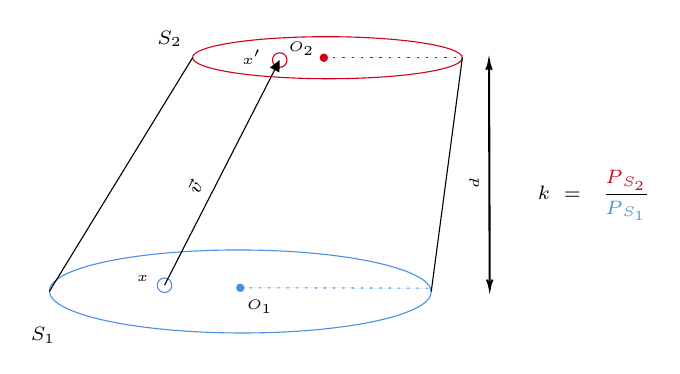
\begin{tikzpicture}[x=0.75pt,y=0.75pt,yscale=-1,xscale=1]
%uncomment if require: \path (0,300); %set diagram left start at 0, and has height of 300

%Shape: Ellipse [id:dp5388131408233692] 
\draw  [color={rgb, 255:red, 208; green, 2; blue, 27 }  ,draw opacity=1 ] (297.51,88.88) .. controls (297.23,83.28) and (326.1,78.75) .. (361.99,78.75) .. controls (397.89,78.75) and (427.21,83.28) .. (427.49,88.88) .. controls (427.77,94.47) and (398.9,99) .. (363.01,99) .. controls (327.11,99) and (297.79,94.47) .. (297.51,88.88) -- cycle ;
%Shape: Ellipse [id:dp777621474822027] 
\draw  [color={rgb, 255:red, 74; green, 144; blue, 226 }  ,draw opacity=1 ] (228.5,201.5) .. controls (227.95,190.45) and (268.69,181.5) .. (319.5,181.5) .. controls (370.31,181.5) and (411.95,190.45) .. (412.5,201.5) .. controls (413.05,212.55) and (372.31,221.5) .. (321.5,221.5) .. controls (270.69,221.5) and (229.05,212.55) .. (228.5,201.5) -- cycle ;
%Straight Lines [id:da6429244999105203] 
\draw    (297.51,88.88) -- (228.5,201.5) ;
%Straight Lines [id:da7997251507611736] 
\draw    (427.49,88.88) -- (412.5,201.5) ;
%Shape: Circle [id:dp47840542367844163] 
\draw  [color={rgb, 255:red, 208; green, 2; blue, 27 }  ,draw opacity=1 ] (336,90) .. controls (336,88.07) and (337.57,86.5) .. (339.5,86.5) .. controls (341.43,86.5) and (343,88.07) .. (343,90) .. controls (343,91.93) and (341.43,93.5) .. (339.5,93.5) .. controls (337.57,93.5) and (336,91.93) .. (336,90) -- cycle ;
%Shape: Circle [id:dp9835136469560248] 
\draw  [color={rgb, 255:red, 74; green, 144; blue, 226 }  ,draw opacity=1 ] (280.5,198.5) .. controls (280.5,196.57) and (282.07,195) .. (284,195) .. controls (285.93,195) and (287.5,196.57) .. (287.5,198.5) .. controls (287.5,200.43) and (285.93,202) .. (284,202) .. controls (282.07,202) and (280.5,200.43) .. (280.5,198.5) -- cycle ;
%Shape: Circle [id:dp283439076913375] 
\draw  [color={rgb, 255:red, 74; green, 144; blue, 226 }  ,draw opacity=1 ][fill={rgb, 255:red, 74; green, 144; blue, 226 }  ,fill opacity=1 ] (318.75,199.75) .. controls (318.75,198.78) and (319.53,198) .. (320.5,198) .. controls (321.47,198) and (322.25,198.78) .. (322.25,199.75) .. controls (322.25,200.72) and (321.47,201.5) .. (320.5,201.5) .. controls (319.53,201.5) and (318.75,200.72) .. (318.75,199.75) -- cycle ;
%Straight Lines [id:da48707589962772135] 
\draw [color={rgb, 255:red, 74; green, 144; blue, 226 }  ,draw opacity=1 ][fill={rgb, 255:red, 74; green, 144; blue, 226 }  ,fill opacity=1 ] [dash pattern={on 0.84pt off 2.51pt}]  (320.5,199.75) -- (412.5,199.88) ;
%Shape: Circle [id:dp49021214062686846] 
\draw  [color={rgb, 255:red, 208; green, 2; blue, 27 }  ,draw opacity=1 ][fill={rgb, 255:red, 208; green, 2; blue, 27 }  ,fill opacity=1 ] (359,88.88) .. controls (359,87.91) and (359.78,87.13) .. (360.75,87.13) .. controls (361.72,87.13) and (362.5,87.91) .. (362.5,88.88) .. controls (362.5,89.84) and (361.72,90.63) .. (360.75,90.63) .. controls (359.78,90.63) and (359,89.84) .. (359,88.88) -- cycle ;
%Straight Lines [id:da1367202995891349] 
\draw [color={rgb, 255:red, 208; green, 2; blue, 27 }  ,draw opacity=1 ][fill={rgb, 255:red, 74; green, 144; blue, 226 }  ,fill opacity=1 ] [dash pattern={on 0.84pt off 2.51pt}]  (360.75,88.88) -- (427.49,88.88) ;
%Straight Lines [id:da5349865593191481] 
\draw    (284,198.5) -- (338.13,92.67) ;
\draw [shift={(339.5,90)}, rotate = 117.09] [fill={rgb, 255:red, 0; green, 0; blue, 0 }  ][line width=0.08]  [draw opacity=0] (5.36,-2.57) -- (0,0) -- (5.36,2.57) -- cycle    ;
%Straight Lines [id:da26724130845467164] 
\draw [line width=0.75]    (440.34,92.33) -- (440.48,139.83) -- (440.5,144.17) -- (440.66,198.17) ;
\draw [shift={(440.67,200.17)}, rotate = 269.83] [color={rgb, 255:red, 0; green, 0; blue, 0 }  ][line width=0.75]    (4.37,-1.32) .. controls (2.78,-0.56) and (1.32,-0.12) .. (0,0) .. controls (1.32,0.12) and (2.78,0.56) .. (4.37,1.32)   ;
\draw [shift={(440.33,90.33)}, rotate = 89.83] [color={rgb, 255:red, 0; green, 0; blue, 0 }  ][line width=0.75]    (4.37,-1.32) .. controls (2.78,-0.56) and (1.32,-0.12) .. (0,0) .. controls (1.32,0.12) and (2.78,0.56) .. (4.37,1.32)   ;

% Text Node
\draw (218.33,217.67) node [anchor=north west][inner sep=0.75pt]  [font=\scriptsize] [align=left] {$\displaystyle S_{1}$};
% Text Node
\draw (279.33,74.67) node [anchor=north west][inner sep=0.75pt]  [font=\scriptsize] [align=left] {$\displaystyle S_{2}$};
% Text Node
\draw (269.53,192.73) node [anchor=north west][inner sep=0.75pt]  [font=\tiny] [align=left] {$\displaystyle x$};
% Text Node
\draw (320.33,84) node [anchor=north west][inner sep=0.75pt]  [font=\tiny] [align=left] {$\displaystyle x'$};
% Text Node
\draw (429.48,152.88) node [anchor=north west][inner sep=0.75pt]  [font=\tiny,rotate=-271.92] [align=left] {$\displaystyle d$};
% Text Node
\draw (462.67,142) node [anchor=north west][inner sep=0.75pt]  [font=\scriptsize] [align=left] {$\displaystyle k\ =\ \ \frac{\textcolor[rgb]{0.82,0.01,0.11}{P}\textcolor[rgb]{0.82,0.01,0.11}{_{S_{2}}}}{\textcolor[rgb]{0.29,0.56,0.89}{P}\textcolor[rgb]{0.29,0.56,0.89}{_{S_{1}}}}$};
% Text Node
\draw (292.58,152.91) node [anchor=north west][inner sep=0.75pt]  [font=\scriptsize,rotate=-296.11] [align=left] {$\displaystyle \vec{v}$};
% Text Node
\draw (322.5,204.5) node [anchor=north west][inner sep=0.75pt]  [font=\tiny] [align=left] {$\displaystyle O_{1}$};
% Text Node
\draw (342.69,80.01) node [anchor=north west][inner sep=0.75pt]  [font=\tiny] [align=left] {$\displaystyle O_{2}$};


\end{tikzpicture}

    \caption{Graphical representation of the growing vector.}
    \label{fig:growing_vector}
\end{figure}

The geometries whose section increases or decreases along the vertical axis also use the factor $k$ to modify the simplices returned by the tessellation algorithm to keep the density of polygons constant in each section.
Although for that purpose, the number of simplices to be obtained is calculated as the product of the number of simplices of the previous layer and the square of the ratio of perimeters.
Taking advantage of the fact that the \textit{trimesh} library is used to read the \textit{STL} file, the \textit{section} function is used to calculate the section of the volume at a given height, \textit{z}, and the \textit{length} property of this section to obtain its perimeter.


\subsection{Shell and structure connection}\label{subsec:shell_struct_connection}

At this point, the core of the structure is finally obtained, and an example of the final structure is shown in the \textcolor{blue}{Figure} \ref{fig:final_structure}.
In the figure, it can be seen that the structure has some floating points, which are the points that have been taken from the shell of the geometry in order to adapt the structure to the geometry.
In this way, the structure has no physical sense, and therefore, it has to be ensured that these points have a connection to other points, both above and below.
To do this, the most obvious option is to connect the points of the shell to each other. 
Thus, as the floating points are part of the shell, it would ensure that they are supported.
For this purpose, the lateral points of the shell are isolated from the rest and iterated over.
For each of these points, its closest points that are above itself and within twice the mean length of the lateral points are retrieved.
From these retrieved points, it is checked if the connection meets the angular condition.
If the connection intersects any other existing edge, and if the connection does not cross any edge closer than the minimum distance allowed.
To check if a connection intersects, or crosses, any edge, the developed algorithm explained in the \textcolor{red}{previous section} is used.
If all the conditions are met, the connection is added to the structure.
For the shell shown in the \textcolor{blue}{Figure} \ref{fig:final_structure}, the connections are shown in the \textcolor{blue}{Figure} \ref{fig:shell_connections} \textcolor{blue}{A}.
For better comprehension of the figure, only the connections between the lateral points are shown.
From the figure, it can be observed that this method is not good enough, as the number of connections depends on the number of points in the surface, which can be very high depending on the meshing parameters used for the geometry.
In addition, it cannot be guaranteed that the connections form a continuous structure, as can be seen in the figure, because the agglomeration of points may mean that the distance conditions are not met, or that some points do not meet the angular condition.
Although at first glance it may seem that they do. On the other hand, the large number of connections can make it computationally very expensive to generate these connections.
Therefore, a good option to reduce the number of connections might be to use only the shell points that are used during the generation of the structure as lateral points.
But, as it can be seen in the \textcolor{blue}{Figure} \ref{fig:shell_connections} \textcolor{blue}{B}, the connections are not enough to ensure that the structure is continuous.
It might be because of the distance between points or their relative position.

\begin{figure}[!htbp]
    \centering
    \begin{subfigure}[b]{0.6\textwidth}
        \centering
        \\includegraphics[width=\textwidth]{imgs/shell.svg.pdf}
        \caption{Connections between the lateral points of the shell.}
    \end{subfigure}
    \begin{subfigure}[b]{0.6\textwidth}
        \centering
        \\includegraphics[width=\textwidth]{imgs/shell_2.svg.pdf}
        \caption{Connections between the lateral points of the shell that are used as lateral points during the generation of the structure.}
    \end{subfigure}
    \caption{Example of the connections between the lateral points of the shell. } 
    \label{fig:shell_connections}
\end{figure}


To solve this issue, several methods, or variations of the methods mentioned above, were studied, but none of them were able to ensure that the structure was continuous.
The only method that ensured the continuity of the structure was to shift the outer points of each layer to the shell, thereby merging both.
Since these points are connected to other points both above and below, when moving them to the shell, these connections will remain, so the structure will be continuous.
The problem with this method is that when the points are shifted, the angular condition may not be fulfilled.
To avoid such situations, it was analysed how much these points are usually displaced to see how much their angles could vary to compensate for this potential variation.
Various geometries were analysed, and it was found that, in general, the displaced distance is about 30 \% of the pore radius, with maximum displacements of 50 \%.
The angle variation due to this displacement can be calculated geometrically as follows.
Consider a general situation such as the one shown in the \textcolor{blue}{Figure} \ref{fig:angle_variation}. 
Since the points are moved to the shell, the closest point between any point and the shell is the projection of the point on the shell. 
Thus, the position of this point in the shell is calculated by projecting the point on the shell, so the displacement will be always perpendicular to the shell, as it is shown in the figure.
Let $d$ be the distance between the point and the shell, $h$ the length of the edge, and $\alpha_1$ the angle of the edge with the horizontal plane, these three values are known a priori.
As mentioned, the point displacement is horizontal so $y = h\sin(\alpha_1)$ will remain constant, and the component $x = h\cos(\alpha_1)$ will increase by $d$.
Then, the following equation can be written:

\begin{equation}
    \begin{aligned}
        \alpha_2 = \arctan \left (\frac{h\sin(\alpha_1)}{h\cos(\alpha_1) + d} \right )
    \end{aligned}
    \label{eq:angle_variation}  
\end{equation}

And the angle variation, $\Delta\alpha$, can be calculated as $\Delta\alpha = \alpha_2 - \alpha_1$. 
Using the structure from the \textcolor{blue}{Figure} \ref{fig:final_structure} as an example, its mean value of the length of the edges and the displacements produced is approximately 8 $mm$ and 1.6 $mm$, respectively, with a maximum displacement of 2.5 $mm$ using a pore radius of 5 $mm$.
Thus, the mean angle variation calculated is $\Delta\alpha = 5 ^\circ $, and $\Delta\alpha = 10 ^\circ$ for the maximum displacement.
Therefore, to compensate for this variation, the angular condition is increased by 10$^\circ$ to avoid breaking the angularity condition when the outer points move towards the shell to be able to use the last-mentioned method.

\begin{figure}[!htbp]
    \centering
    

\tikzset{every picture/.style={line width=0.75pt}} %set default line width to 0.75pt        

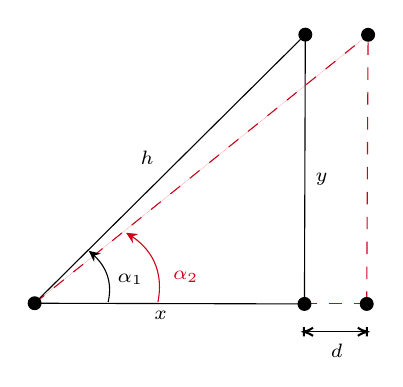
\begin{tikzpicture}[x=0.75pt,y=0.75pt,yscale=-1,xscale=1]
%uncomment if require: \path (0,300); %set diagram left start at 0, and has height of 300

%Straight Lines [id:da607447387383602] 
\draw [color={rgb, 255:red, 208; green, 2; blue, 27 }  ,draw opacity=1 ][fill={rgb, 255:red, 230; green, 39; blue, 39 }  ,fill opacity=1 ] [dash pattern={on 4.5pt off 4.5pt}]  (195.25,185.75) -- (355.92,56.42) ;
%Straight Lines [id:da27148655997396476] 
\draw [color={rgb, 255:red, 208; green, 2; blue, 27 }  ,draw opacity=1 ] [dash pattern={on 4.5pt off 4.5pt}]  (355.25,186.08) -- (355.92,56.42) ;
%Straight Lines [id:da7571554100323626] 
\draw [color={rgb, 255:red, 208; green, 2; blue, 27 }  ,draw opacity=1 ] [dash pattern={on 4.5pt off 4.5pt}]  (325.25,186.08) -- (355.25,186.08) ;
%Shape: Circle [id:dp7176360013947902] 
\draw  [fill={rgb, 255:red, 0; green, 0; blue, 0 }  ,fill opacity=1 ] (192.17,185.75) .. controls (192.17,184.05) and (193.55,182.67) .. (195.25,182.67) .. controls (196.95,182.67) and (198.33,184.05) .. (198.33,185.75) .. controls (198.33,187.45) and (196.95,188.83) .. (195.25,188.83) .. controls (193.55,188.83) and (192.17,187.45) .. (192.17,185.75) -- cycle ;
%Shape: Circle [id:dp24601699255953835] 
\draw  [fill={rgb, 255:red, 0; green, 0; blue, 0 }  ,fill opacity=1 ] (322.17,186.08) .. controls (322.17,184.38) and (323.55,183) .. (325.25,183) .. controls (326.95,183) and (328.33,184.38) .. (328.33,186.08) .. controls (328.33,187.79) and (326.95,189.17) .. (325.25,189.17) .. controls (323.55,189.17) and (322.17,187.79) .. (322.17,186.08) -- cycle ;
%Shape: Circle [id:dp906352155237646] 
\draw  [fill={rgb, 255:red, 0; green, 0; blue, 0 }  ,fill opacity=1 ] (322.58,56.33) .. controls (322.58,54.63) and (323.96,53.25) .. (325.67,53.25) .. controls (327.37,53.25) and (328.75,54.63) .. (328.75,56.33) .. controls (328.75,58.04) and (327.37,59.42) .. (325.67,59.42) .. controls (323.96,59.42) and (322.58,58.04) .. (322.58,56.33) -- cycle ;
%Straight Lines [id:da11648942189495237] 
\draw    (195.25,185.75) -- (325.67,56.33) ;
%Straight Lines [id:da26461786666325793] 
\draw    (195.25,185.75) -- (325.25,186.08) ;
%Straight Lines [id:da23855514855400362] 
\draw    (325.25,186.08) -- (325.67,56.33) ;
%Curve Lines [id:da7632155654947097] 
\draw    (230.67,185.17) .. controls (233.4,173.41) and (227.62,166.14) .. (223.61,162.44) ;
\draw [shift={(221.33,160.5)}, rotate = 38.66] [fill={rgb, 255:red, 0; green, 0; blue, 0 }  ][line width=0.08]  [draw opacity=0] (5.36,-2.57) -- (0,0) -- (5.36,2.57) -- (3.56,0) -- cycle    ;
%Shape: Circle [id:dp2379888459592604] 
\draw  [fill={rgb, 255:red, 0; green, 0; blue, 0 }  ,fill opacity=1 ] (352.17,186.08) .. controls (352.17,184.38) and (353.55,183) .. (355.25,183) .. controls (356.95,183) and (358.33,184.38) .. (358.33,186.08) .. controls (358.33,187.79) and (356.95,189.17) .. (355.25,189.17) .. controls (353.55,189.17) and (352.17,187.79) .. (352.17,186.08) -- cycle ;
%Shape: Circle [id:dp4318264592938509] 
\draw  [fill={rgb, 255:red, 0; green, 0; blue, 0 }  ,fill opacity=1 ] (352.83,56.42) .. controls (352.83,54.71) and (354.21,53.33) .. (355.92,53.33) .. controls (357.62,53.33) and (359,54.71) .. (359,56.42) .. controls (359,58.12) and (357.62,59.5) .. (355.92,59.5) .. controls (354.21,59.5) and (352.83,58.12) .. (352.83,56.42) -- cycle ;
%Curve Lines [id:da5116933081563226] 
\draw [color={rgb, 255:red, 208; green, 2; blue, 27 }  ,draw opacity=1 ]   (254.67,185.17) .. controls (258.31,166.13) and (247.36,156.97) .. (241.79,153.34) ;
\draw [shift={(239.33,151.83)}, rotate = 30.96] [fill={rgb, 255:red, 208; green, 2; blue, 27 }  ,fill opacity=1 ][line width=0.08]  [draw opacity=0] (5.36,-2.57) -- (0,0) -- (5.36,2.57) -- (3.56,0) -- cycle    ;
%Straight Lines [id:da10028566006612083] 
\draw    (325,199.5) -- (355.33,199.5) ;
\draw [shift={(355.33,199.5)}, rotate = 180] [color={rgb, 255:red, 0; green, 0; blue, 0 }  ][line width=0.75]    (0,2.24) -- (0,-2.24)(4.37,-1.96) .. controls (2.78,-0.92) and (1.32,-0.27) .. (0,0) .. controls (1.32,0.27) and (2.78,0.92) .. (4.37,1.96)   ;
\draw [shift={(325,199.5)}, rotate = 0] [color={rgb, 255:red, 0; green, 0; blue, 0 }  ][line width=0.75]    (0,2.24) -- (0,-2.24)(4.37,-1.96) .. controls (2.78,-0.92) and (1.32,-0.27) .. (0,0) .. controls (1.32,0.27) and (2.78,0.92) .. (4.37,1.96)   ;

% Text Node
\draw (234,170.33) node [anchor=north west][inner sep=0.75pt]  [font=\scriptsize] [align=left] {$\displaystyle \alpha _{1}$};
% Text Node
\draw (260.67,169) node [anchor=north west][inner sep=0.75pt]  [font=\scriptsize] [align=left] {$\displaystyle \textcolor[rgb]{0.82,0.01,0.11}{\alpha }\textcolor[rgb]{0.82,0.01,0.11}{_{2}}$};
% Text Node
\draw (336.67,204) node [anchor=north west][inner sep=0.75pt]  [font=\scriptsize] [align=left] {$\displaystyle d$};
% Text Node
\draw (251.67,188.33) node [anchor=north west][inner sep=0.75pt]  [font=\scriptsize] [align=left] {$\displaystyle x$};
% Text Node
\draw (329.33,122) node [anchor=north west][inner sep=0.75pt]  [font=\scriptsize] [align=left] {$\displaystyle y$};
% Text Node
\draw (245,111) node [anchor=north west][inner sep=0.75pt]  [font=\scriptsize] [align=left] {$\displaystyle h$};


\end{tikzpicture}

    \caption{Point to shell displacement diagram.}
    \label{fig:angle_variation}
\end{figure}

\subsection{Termination condition}\label{sec:termination_cond}

Each time a new vertex is generated, it is checked if it is inside the volume. 
If it is, the vertex is added as a new vertex that will serve as a base point for the next layer's polygons.
If not, that means that the top of the volume has been reached, so the vertex is not added as a new vertex.
Due to the fact that the heights of the tetrahedron in each layer are not equal, finding a proposed vertex that lies outside the volume does not mean that the top of the volume has been reached for the rest of the vertices.
So, the algorithm will continue to generate vertices until all the proposed vertices are outside the volume.

It would be expected that when a polygon generates a vertex that is outside the volume, it should be removed so that it does not constantly generate an invalid vertex. 
But if the polygon is eliminated, or rather, if the points that form that polygon are not considered for future layers, what is actually being done is to reduce the number of points for the following layers and, therefore, generating other tetrahedra on top of these points, which may cause intersections between the edges. 
Moreover, this would lead to a loss of continuity of the structure, as the points that are not considered will not be connected to any other points above them. This issue is illustrated in \textcolor{blue}{Figure} \ref{fig:draft_termination}.

\begin{figure}[h]
  \centering
  \includegraphics[width=0.8\textwidth]{imgs/Figure_8.png}
  \caption{ A) Example of a set of tetrahedra formed from a set of (delineated) bases. Bases that do not have a vertex represent bases that generate a vertex that is outside the volume. B) Example of bases obtained in the next layer without using the proposed logic. Here, as can be seen, there are certain points of the previous layer that are isolated, causing a loss of continuity. C) Example of bases obtained in the following layer of triangles, considering the bases that have not been able to generate the vertex of the previous layer.}
  \label{fig:draft_termination}
\end{figure}


In the \textcolor{blue}{Figure} \ref{fig:termination} is shown a graphical representation of this termination condition.
The orange points in the \textcolor{blue}{Figure} \ref{fig:termination} \textcolor{blue}{A} represent the points of the penultimate layer, and the red points represent the vertexes generated from this layer.
As can be seen, the difference in the heights of the points of the layers causes the highest polygons not to generate a vertex because it would lie outside the volume.
That is why the zone at the back is empty of red points.
But, as mentioned above, the polygons that do not generate points are still considered for the next layer, so the vertex generated previously are connected to the base points that did not generate a vertex, as shown in the \textcolor{blue}{Figure} \ref{fig:termination} \textcolor{blue}{B}. 
This ensures that the structure is continuous and that the edges do not intersect.
Once all the polygons in a layer can no longer generate a vertex, the algorithm stops, and the points of the structure that have no connection above them are moved to the top of the volume, so the structure is closed.
It could seem that by doing this, the angular condition can be violated, but it is not, since the points are moving vertically, and the angles can only increase.

\begin{figure}[!htbp]
    \centering
    \begin{subfigure}[b]{0.49\textwidth}
        \centering
        \\includegraphics[width=\textwidth]{imgs/prelast.svg.pdf}
        \caption{Penultimate layer}
    \end{subfigure}
    \begin{subfigure}[b]{0.49\textwidth}
        \centering
        \\includegraphics[width=\textwidth]{imgs/last.svg.pdf}
        \caption{Last layer}
    \end{subfigure}
    \caption{Example of the two last layers of a structure. Image \textbf{A} shows the points of the penultimate layer in orange and the vertices generated from this layer in red. Image \textbf{B} shows the last layer obtained from the vertices generated in the previous layer and the base points that did not generate a vertex; no vertices are generated from this layer because all would lie outside the volume. Grey points in both images represent the top points of the volume.}
    \label{fig:termination}
\end{figure}

In addition, it was observed that some points generated outside the volume were too close to the upper surface and were discarded because they were outside. This caused the tetrahedra of the last layer to be very long and, therefore, their edges. 
To improve this behaviour, a routine was implemented that assessed whether these points could be moved vertically to the surface without breaking the angularity condition. 
To do so, when a vertex is generated outside the volume, the minimum angle of the edges of its tetrahedron is retrieved. 
Then, the maximum vertical displacement allowed by this edge is calculated using the \textcolor{blue}{Equation} \ref{eq:delta-deduccion}. 
The maximum permissible vertical displacement is understood to be the displacement of the candidate point that causes the edge angle to be 45$^{\circ}$. 
A graphical explanation of the maximum displacement allowed is shown in \textcolor{blue}{Figure} \ref{fig:termination_demons}.

\begin{figure}[!htbp]
  \centering
  \begin{minipage}[t]{0.4\textwidth}\vspace{0pt}
    \centering
    

\tikzset{every picture/.style={line width=0.75pt}} %set default line width to 0.75pt        

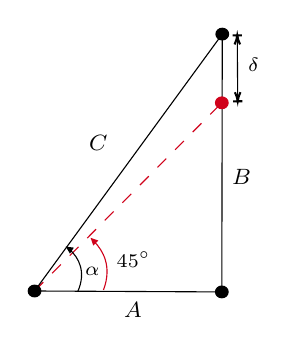
\begin{tikzpicture}[x=0.75pt,y=0.75pt,yscale=-1,xscale=1]
%uncomment if require: \path (0,300); %set diagram left start at 0, and has height of 300

%Straight Lines [id:da20080091364174113] 
\draw [color={rgb, 255:red, 208; green, 2; blue, 27 }  ,draw opacity=1 ] [dash pattern={on 4.5pt off 4.5pt}]  (59.94,139.84) -- (150.16,49.17) ;
%Straight Lines [id:da7666578220448256] 
\draw    (150.16,140.29) -- (150.27,79.78) -- (150.38,16.06) ;
%Flowchart: Connector [id:dp25706287258768046] 
\draw  [fill={rgb, 255:red, 0; green, 0; blue, 0 }  ,fill opacity=1 ] (56.89,139.84) .. controls (56.89,138.28) and (58.25,137.02) .. (59.94,137.02) .. controls (61.62,137.02) and (62.99,138.28) .. (62.99,139.84) .. controls (62.99,141.4) and (61.62,142.67) .. (59.94,142.67) .. controls (58.25,142.67) and (56.89,141.4) .. (56.89,139.84) -- cycle ;
%Flowchart: Connector [id:dp7129901164482209] 
\draw  [fill={rgb, 255:red, 0; green, 0; blue, 0 }  ,fill opacity=1 ] (147.11,140.29) .. controls (147.11,138.73) and (148.48,137.46) .. (150.16,137.46) .. controls (151.85,137.46) and (153.21,138.73) .. (153.21,140.29) .. controls (153.21,141.85) and (151.85,143.11) .. (150.16,143.11) .. controls (148.48,143.11) and (147.11,141.85) .. (147.11,140.29) -- cycle ;
%Flowchart: Connector [id:dp14605193492059754] 
\draw  [color={rgb, 255:red, 208; green, 2; blue, 27 }  ,draw opacity=1 ][fill={rgb, 255:red, 208; green, 2; blue, 27 }  ,fill opacity=1 ] (147.11,49.17) .. controls (147.11,47.61) and (148.48,46.35) .. (150.16,46.35) .. controls (151.85,46.35) and (153.21,47.61) .. (153.21,49.17) .. controls (153.21,50.74) and (151.85,52) .. (150.16,52) .. controls (148.48,52) and (147.11,50.74) .. (147.11,49.17) -- cycle ;
%Flowchart: Connector [id:dp3770909275464782] 
\draw  [fill={rgb, 255:red, 0; green, 0; blue, 0 }  ,fill opacity=1 ] (147.33,16.06) .. controls (147.33,14.5) and (148.7,13.24) .. (150.38,13.24) .. controls (152.07,13.24) and (153.43,14.5) .. (153.43,16.06) .. controls (153.43,17.62) and (152.07,18.89) .. (150.38,18.89) .. controls (148.7,18.89) and (147.33,17.62) .. (147.33,16.06) -- cycle ;
%Straight Lines [id:da4689098365411484] 
\draw    (59.94,139.84) -- (150.16,140.29) ;
%Straight Lines [id:da7092156895773364] 
\draw    (59.94,139.84) -- (150.38,16.06) ;
%Curve Lines [id:da4859163134212995] 
\draw [color={rgb, 255:red, 208; green, 2; blue, 27 }  ,draw opacity=1 ]   (93.16,139.33) .. controls (97.5,127.56) and (92.55,120.22) .. (89,116.34) ;
\draw [shift={(86.93,114.22)}, rotate = 45] [fill={rgb, 255:red, 208; green, 2; blue, 27 }  ,fill opacity=1 ][line width=0.08]  [draw opacity=0] (3.57,-1.72) -- (0,0) -- (3.57,1.72) -- cycle    ;
%Straight Lines [id:da6280238401163977] 
\draw    (157.6,16.67) -- (157.82,48.44) ;
\draw [shift={(157.82,48.44)}, rotate = 269.6] [color={rgb, 255:red, 0; green, 0; blue, 0 }  ][line width=0.75]    (0,2.24) -- (0,-2.24)(4.37,-1.32) .. controls (2.78,-0.56) and (1.32,-0.12) .. (0,0) .. controls (1.32,0.12) and (2.78,0.56) .. (4.37,1.32)   ;
\draw [shift={(157.6,16.67)}, rotate = 89.6] [color={rgb, 255:red, 0; green, 0; blue, 0 }  ][line width=0.75]    (0,2.24) -- (0,-2.24)(4.37,-1.32) .. controls (2.78,-0.56) and (1.32,-0.12) .. (0,0) .. controls (1.32,0.12) and (2.78,0.56) .. (4.37,1.32)   ;
%Curve Lines [id:da9497681171147138] 
\draw [color={rgb, 255:red, 0; green, 0; blue, 0 }  ,draw opacity=1 ]   (80.71,140.22) .. controls (85.08,130.38) and (80.94,123.68) .. (77.22,120.24) ;
\draw [shift={(74.93,118.44)}, rotate = 32.91] [fill={rgb, 255:red, 0; green, 0; blue, 0 }  ,fill opacity=1 ][line width=0.08]  [draw opacity=0] (3.57,-1.72) -- (0,0) -- (3.57,1.72) -- cycle    ;

% Text Node
\draw (90.04,130.54) node  [font=\scriptsize] [align=left] {\begin{minipage}[lt]{8.67pt}\setlength\topsep{0pt}
$\displaystyle \alpha $
\end{minipage}};
% Text Node
\draw (98.27,119.43) node [anchor=north west][inner sep=0.75pt]  [font=\scriptsize] [align=left] {$\displaystyle 45^{\circ }$};
% Text Node
\draw (84.93,63.6) node [anchor=north west][inner sep=0.75pt]  [font=\footnotesize] [align=left] {$\displaystyle C$};
% Text Node
\draw (101.82,144.04) node [anchor=north west][inner sep=0.75pt]  [font=\footnotesize] [align=left] {$\displaystyle A$};
% Text Node
\draw (153.82,80.04) node [anchor=north west][inner sep=0.75pt]  [font=\footnotesize] [align=left] {$\displaystyle B$};
% Text Node
\draw (161.6,26.49) node [anchor=north west][inner sep=0.75pt]  [font=\scriptsize] [align=left] {$\displaystyle \delta$};


\end{tikzpicture}

    \caption{Geometric explanation of the maximum displacement allowed ($\delta$) for the nodes outside the volume.}
    \label{fig:termination_demons}
  \end{minipage}%
  \hfill
  \begin{minipage}[t]{0.4\textwidth}\vspace{0pt}
    \centering
    \begin{align}
        B' &= B - \delta &&\Rightarrow && \delta = B - B' \nonumber \\
        \tan(\alpha) &= \frac{B}{A} &&\Rightarrow && B = A \tan(\alpha) \nonumber \\
        \tan(\alpha') &= \frac{B'}{A} &&\Rightarrow && B' = A \tan(\alpha') \nonumber \\
        &&&\Rightarrow && \delta = A\left(\tan(\alpha) - \cancelto{1}{\tan(\alpha')}\right) \label{eq:delta-deduccion}
    \end{align}
  \end{minipage}
\end{figure}

In the \textcolor{blue}{Figure} \ref{fig:final_structure}, a comparison between before and after implementing this improvement is shown. It can be observed that the number of layers and points in the upper area of the volume increases, thus reducing the length of the struts in the upper layers. \textcolor{blue}{Figure} \ref{fig:final_structure} 
\textcolor{blue}{B} also shows an example of the final graph-like structure obtained from this methodology. Once it is finished, the object obtained is converted into a \textit{NetworkX's} \footnote{\href{https://networkx.org/}{NetworkX} is a Python package for the creation, manipulation, and study of the structure, dynamics, and functions of complex networks.} graph. During this process, all edges of the structure are rechecked to ensure that they meet all conditions. If not, the problems are eliminated.


\begin{figure}[!htbp]
    \centering
    \begin{subfigure}[b]{0.45\textwidth}
        \centering
        \\includegraphics[width=\textwidth]{imgs/Figure_20.svg.pdf}
        \caption{Before improvement}
    \end{subfigure}
    \begin{subfigure}[b]{0.47\textwidth}
        \centering
        \\includegraphics[width=\textwidth]{imgs/Figure_1.svg.pdf}
        \caption{After improvement}
    \end{subfigure}
    \caption{Comparison of two structures obtained before and after implementing the logic to improve the behaviour of the termination criteria routine. Image \textbf{A} shows a structure obtained without considering outside points as possible candidates. Image \textbf{B} shows a structure obtained after considering outside points as possible candidates.}
    \label{fig:final_structure}
\end{figure}


\end{document}